% Options for packages loaded elsewhere
% Options for packages loaded elsewhere
\PassOptionsToPackage{unicode}{hyperref}
\PassOptionsToPackage{hyphens}{url}
\PassOptionsToPackage{dvipsnames,svgnames,x11names}{xcolor}
%
\documentclass[
  letterpaper,
  DIV=11,
  numbers=noendperiod,
  12pt]{scrartcl}
\usepackage{xcolor}
\usepackage{amsmath,amssymb}
\setcounter{secnumdepth}{-\maxdimen} % remove section numbering
\usepackage{iftex}
\ifPDFTeX
  \usepackage[T1]{fontenc}
  \usepackage[utf8]{inputenc}
  \usepackage{textcomp} % provide euro and other symbols
\else % if luatex or xetex
  \usepackage{unicode-math} % this also loads fontspec
  \defaultfontfeatures{Scale=MatchLowercase}
  \defaultfontfeatures[\rmfamily]{Ligatures=TeX,Scale=1}
\fi
\usepackage{lmodern}
\ifPDFTeX\else
  % xetex/luatex font selection
\fi
% Use upquote if available, for straight quotes in verbatim environments
\IfFileExists{upquote.sty}{\usepackage{upquote}}{}
\IfFileExists{microtype.sty}{% use microtype if available
  \usepackage[]{microtype}
  \UseMicrotypeSet[protrusion]{basicmath} % disable protrusion for tt fonts
}{}
\usepackage{setspace}
\makeatletter
\@ifundefined{KOMAClassName}{% if non-KOMA class
  \IfFileExists{parskip.sty}{%
    \usepackage{parskip}
  }{% else
    \setlength{\parindent}{0pt}
    \setlength{\parskip}{6pt plus 2pt minus 1pt}}
}{% if KOMA class
  \KOMAoptions{parskip=half}}
\makeatother
% Make \paragraph and \subparagraph free-standing
\makeatletter
\ifx\paragraph\undefined\else
  \let\oldparagraph\paragraph
  \renewcommand{\paragraph}{
    \@ifstar
      \xxxParagraphStar
      \xxxParagraphNoStar
  }
  \newcommand{\xxxParagraphStar}[1]{\oldparagraph*{#1}\mbox{}}
  \newcommand{\xxxParagraphNoStar}[1]{\oldparagraph{#1}\mbox{}}
\fi
\ifx\subparagraph\undefined\else
  \let\oldsubparagraph\subparagraph
  \renewcommand{\subparagraph}{
    \@ifstar
      \xxxSubParagraphStar
      \xxxSubParagraphNoStar
  }
  \newcommand{\xxxSubParagraphStar}[1]{\oldsubparagraph*{#1}\mbox{}}
  \newcommand{\xxxSubParagraphNoStar}[1]{\oldsubparagraph{#1}\mbox{}}
\fi
\makeatother


\usepackage{longtable,booktabs,array}
\usepackage{calc} % for calculating minipage widths
% Correct order of tables after \paragraph or \subparagraph
\usepackage{etoolbox}
\makeatletter
\patchcmd\longtable{\par}{\if@noskipsec\mbox{}\fi\par}{}{}
\makeatother
% Allow footnotes in longtable head/foot
\IfFileExists{footnotehyper.sty}{\usepackage{footnotehyper}}{\usepackage{footnote}}
\makesavenoteenv{longtable}
\usepackage{graphicx}
\makeatletter
\newsavebox\pandoc@box
\newcommand*\pandocbounded[1]{% scales image to fit in text height/width
  \sbox\pandoc@box{#1}%
  \Gscale@div\@tempa{\textheight}{\dimexpr\ht\pandoc@box+\dp\pandoc@box\relax}%
  \Gscale@div\@tempb{\linewidth}{\wd\pandoc@box}%
  \ifdim\@tempb\p@<\@tempa\p@\let\@tempa\@tempb\fi% select the smaller of both
  \ifdim\@tempa\p@<\p@\scalebox{\@tempa}{\usebox\pandoc@box}%
  \else\usebox{\pandoc@box}%
  \fi%
}
% Set default figure placement to htbp
\def\fps@figure{htbp}
\makeatother


% definitions for citeproc citations
\NewDocumentCommand\citeproctext{}{}
\NewDocumentCommand\citeproc{mm}{%
  \begingroup\def\citeproctext{#2}\cite{#1}\endgroup}
\makeatletter
 % allow citations to break across lines
 \let\@cite@ofmt\@firstofone
 % avoid brackets around text for \cite:
 \def\@biblabel#1{}
 \def\@cite#1#2{{#1\if@tempswa , #2\fi}}
\makeatother
\newlength{\cslhangindent}
\setlength{\cslhangindent}{1.5em}
\newlength{\csllabelwidth}
\setlength{\csllabelwidth}{3em}
\newenvironment{CSLReferences}[2] % #1 hanging-indent, #2 entry-spacing
 {\begin{list}{}{%
  \setlength{\itemindent}{0pt}
  \setlength{\leftmargin}{0pt}
  \setlength{\parsep}{0pt}
  % turn on hanging indent if param 1 is 1
  \ifodd #1
   \setlength{\leftmargin}{\cslhangindent}
   \setlength{\itemindent}{-1\cslhangindent}
  \fi
  % set entry spacing
  \setlength{\itemsep}{#2\baselineskip}}}
 {\end{list}}
\usepackage{calc}
\newcommand{\CSLBlock}[1]{\hfill\break\parbox[t]{\linewidth}{\strut\ignorespaces#1\strut}}
\newcommand{\CSLLeftMargin}[1]{\parbox[t]{\csllabelwidth}{\strut#1\strut}}
\newcommand{\CSLRightInline}[1]{\parbox[t]{\linewidth - \csllabelwidth}{\strut#1\strut}}
\newcommand{\CSLIndent}[1]{\hspace{\cslhangindent}#1}



\setlength{\emergencystretch}{3em} % prevent overfull lines

\providecommand{\tightlist}{%
  \setlength{\itemsep}{0pt}\setlength{\parskip}{0pt}}



 


\usepackage{booktabs}
\usepackage{longtable}
\usepackage{array}
\usepackage{multirow}
\usepackage{wrapfig}
\usepackage{float}
\usepackage{colortbl}
\usepackage{pdflscape}
\usepackage{tabularx}
\usepackage{xltabular}
\usepackage{threeparttable}
\usepackage{threeparttablex}
\usepackage[normalem]{ulem}
\usepackage{makecell}
\usepackage{xcolor}
\KOMAoption{captions}{tableheading}
\usepackage{setspace}
\doublespacing
\usepackage{lineno}
\linenumbers
\usepackage{threeparttable}
\makeatletter
\@ifpackageloaded{caption}{}{\usepackage{caption}}
\AtBeginDocument{%
\ifdefined\contentsname
  \renewcommand*\contentsname{Table of contents}
\else
  \newcommand\contentsname{Table of contents}
\fi
\ifdefined\listfigurename
  \renewcommand*\listfigurename{List of Figures}
\else
  \newcommand\listfigurename{List of Figures}
\fi
\ifdefined\listtablename
  \renewcommand*\listtablename{List of Tables}
\else
  \newcommand\listtablename{List of Tables}
\fi
\ifdefined\figurename
  \renewcommand*\figurename{Figure}
\else
  \newcommand\figurename{Figure}
\fi
\ifdefined\tablename
  \renewcommand*\tablename{Table}
\else
  \newcommand\tablename{Table}
\fi
}
\@ifpackageloaded{float}{}{\usepackage{float}}
\floatstyle{ruled}
\@ifundefined{c@chapter}{\newfloat{codelisting}{h}{lop}}{\newfloat{codelisting}{h}{lop}[chapter]}
\floatname{codelisting}{Listing}
\newcommand*\listoflistings{\listof{codelisting}{List of Listings}}
\makeatother
\makeatletter
\makeatother
\makeatletter
\@ifpackageloaded{caption}{}{\usepackage{caption}}
\@ifpackageloaded{subcaption}{}{\usepackage{subcaption}}
\makeatother
\usepackage{bookmark}
\IfFileExists{xurl.sty}{\usepackage{xurl}}{} % add URL line breaks if available
\urlstyle{same}
\hypersetup{
  pdftitle={The upstream placebo: reservoir siting, not regulation, explains apparent drought buffering during Chile's megadrought},
  pdfauthor={Francisco Zambrano Bigiarini},
  pdfkeywords={reservoir effect, drought
propagation, socio-hydrology, causal inference, megadrought, Chile},
  colorlinks=true,
  linkcolor={blue},
  filecolor={Maroon},
  citecolor={Blue},
  urlcolor={Blue},
  pdfcreator={LaTeX via pandoc}}


\title{The upstream placebo: reservoir siting, not regulation, explains
apparent drought buffering during Chile's megadrought}
\author{Francisco Zambrano Bigiarini}
\date{2026-08-04}
\begin{document}
\maketitle
\begin{abstract}
Much of what the hydrological literature attributes to reservoir drought
buffering may be a measurable siting confound. We treat reservoir
presence as a basin-level intervention in Chile's megadrought and
separate siting from operation with an upstream/downstream placebo:
regulated reaches below each dam are compared against unregulated
reaches above, which share climate, geology, and selection history but
not the reservoir. Across the streamflow pathway the apparent buffering
is as strong upstream as downstream (differential slopes \(-0.20\)
versus \(-0.16\), randomization-inference \(p = 0.39\)), the signature
of aridity, not regulation. A hard-balanced match forcing aridity to be
identical across groups (standardized mean difference 0.000) makes even
the apparent buffering vanish entirely (intent-to-treat \(-0.02\),
\(p > 0.85\)). The streamflow null is well powered, excluding
operational buffering above 46 to 59\% of baseline, and a positive
control confirms that the design recovers injected effects one to one.
Dammed basins hold 4.5 times more cropland than matched controls, a
siting legacy stable across the 2000 to 2024 record with no detected
megadrought divergence. The storage band drifts downward in step with
the independent decline in unregulated streamflow. Demand-side outcomes,
cropland expansion, water rights accrual, and evapotranspiration, are
consistent with no operational effect but underpowered as stand-alone
tests. Through the megadrought we detect no operational buffering and no
megadrought-era demand expansion beyond the siting legacy. The upstream
placebo is a portable method for regulated rivers with gauges above and
below dams. Adaptation must shift toward managing demand.
\end{abstract}


\setstretch{2}
\section{Introduction}\label{introduction}

A persistent obstacle separates what we think reservoirs do during
drought from what they actually do: dams are built where water is
already scarce, so dammed basins differ systematically from undammed
ones before any drought strikes. The short-term hydrological benefit of
storage is documented (Wu et al. 2017, 2018), but whether reservoirs
buffer multi-year drought, or whether the apparent buffering is a
statistical shadow of where dams sit, has remained untested for want of
a credible counterfactual (Di Baldassarre et al. 2018). The distinction
matters. If buffering is real, expanding storage is a rational
adaptation to intensifying drought. If it is siting, then the reflexive
global response, more dams, invests in the wrong mechanism.

The reservoir-effect hypothesis (Di Baldassarre et al. 2018) formalizes
the concern: greater supply invites expansion, so demand grows to meet
and then exceed each increment of storage (the supply-demand cycle), and
prolonged reliance on stored abundance erodes the incentive to adapt,
magnifying the damage when drought finally outlasts the reservoir.
Consistent with this, global demand has outpaced storage for decades,
returns of new dams are diminishing (Li et al. 2023), and most
reservoirs now fail to refill (Z. Wang et al. 2024). Whether these
feedbacks dominate, or are outweighed by the protection dams provide,
remains debated (Kellner 2021). But the empirical literature has a
structural weakness: dammed-versus-undammed or before-after comparisons
cannot separate a reservoir effect from the siting decision, because
reservoirs concentrate where irrigation demand and aridity already
concentrate.

We address this with a within-basin falsification test. If a dam buffers
drought, streamflow transmission from meteorological to hydrological
drought should flatten only below the dam, where regulation operates. If
it flattens equally at the unregulated upstream reaches of the same
basins, the attenuation is siting, not regulation. This
upstream/downstream placebo is the paper's central identification
strategy. We complement it with a matched cross-basin comparison that
conditions each dammed basin against hydroclimatically comparable
undammed basins, and we evaluate both against the drought each basin
actually experienced rather than against calendar time, breaking the
collinearity between the megadrought onset and the treatment clock.

Chile is an acute testbed. Since 2010 its central regions have endured a
\emph{megadrought}, an uninterrupted run of dry years shading into
structural aridification with a documented anthropogenic component (R.
D. Garreaud et al. 2017; R. Garreaud et al. 2025; Zambrano et al. 2025;
Boisier et al. 2018; Vicente‐Serrano et al. 2019). The 1981 Water Code
makes water-use rights perpetual private property that the state cannot
readily curtail, so the policy reflex has been supply-side: new dams and
inter-basin transfers, alongside market incentives that concentrated
water in high-value export crops (Barría et al. 2021; Reade Malagueño
and D'Odorico 2024; Rivera et al. 2016). In the snow-fed basins of
central Chile demand already outruns supply in roughly three years of
every ten (Webb et al. 2021). Chile thus exhibits every ingredient of
the reservoir effect: extreme persistent forcing, a supply-side
response, and demand expansion under weak adaptive feedback, making it a
most-likely case for detecting a reservoir effect if one operates. At
the same time, its short, steep Andean catchments, with streamflow
gauges above and below major dams, provide the physical setup the
upstream placebo requires, a configuration present across the world's
regulated mountain rivers from the Sierra Nevada to the European Alps to
the African Rift.

We apply this design across four outcome pathways: streamflow drought
transmission, cropland area change, consumptive water-rights accrual,
and evapotranspiration. Throughout, outcomes are evaluated at annual to
multi-year accumulations, the timescale of structural drought, not of
seasonal operation. We find that across the streamflow pathway the
apparent buffering is a siting confound, that the upstream placebo
identifies it, and that the operational effect of reservoirs on drought
brackets zero once siting is matched out. The upstream placebo is a
portable method: wherever rivers have gauges above and below dams, the
same falsification test can separate siting from effect.

\section{Results}\label{results}

\subsection{Reservoirs sit where water is already
scarce}\label{reservoirs-sit-where-water-is-already-scarce}

Reservoirs in Chile are built where drought bites hardest: our 21 dammed
basins cluster in the arid centre and north, so a raw comparison would
confuse the reservoir with its location. We separate them with the
design in Figure~\ref{fig-schematic}. First, we compare each dammed
basin only with undammed basins sharing its climate, size and elevation,
keeping 21 of 24 dammed basins against an effective 91 of 244 controls
(Supplementary Figs. S4 and S5), and we condition on the drought each
basin experienced, comparing impact per unit of deficit. Second, within
each dammed basin we compare regulated reaches below the dam against
unregulated reaches above it. A genuine reservoir effect must appear in
these comparisons; in none does it.

\begin{figure}

\centering{

\pandocbounded{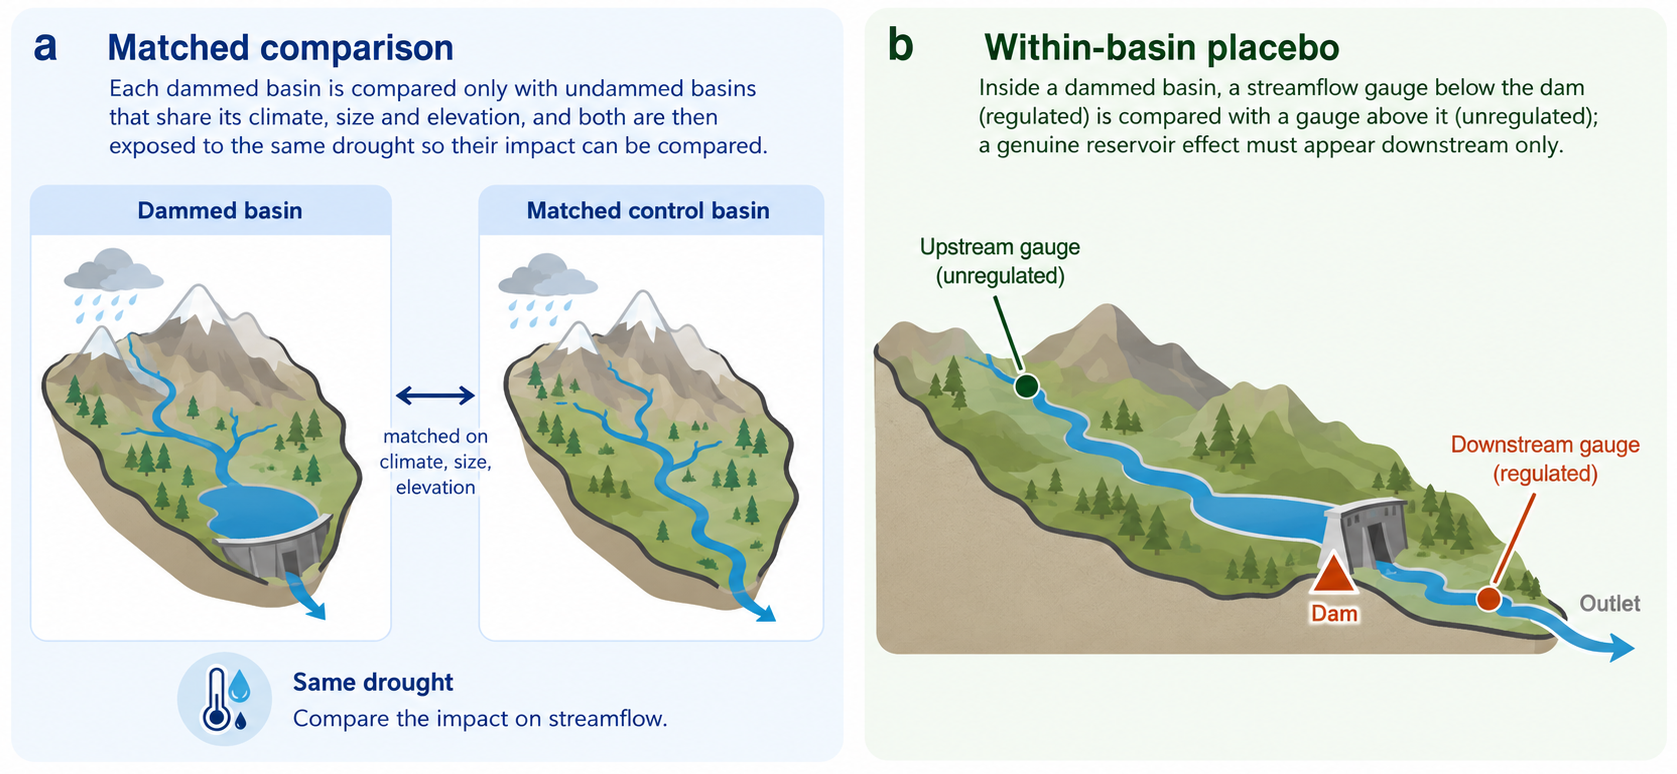
\includegraphics[keepaspectratio]{../../results/figures/fig_design_schematic_v2.png}}

}

\caption{\label{fig-schematic}The two comparisons that separate the
reservoir from its location. (a) Matched comparison: each dammed basin
is compared only with undammed basins that share its climate, size and
elevation, and both are then exposed to the same drought so their impact
can be compared. (b) Within-basin placebo: inside a dammed basin, a
streamflow gauge below the dam (regulated) is compared with a gauge
above it (unregulated); a genuine reservoir effect must appear
downstream only. Schematic; the full study-area map and matching
diagnostics are in Supplementary Figs. S4 and S5.}

\end{figure}%

\subsection{The apparent buffering is the location, not the
dam}\label{sec-placebo}

The most direct test is on streamflow. Meteorological drought
(Standardized Precipitation Evapotranspiration Index of 12 months,
SPEI-12) propagates into streamflow drought (Standardized Streamflow
Index of 12 months, SSI-12) more gently in dammed basins, the visual
signature of buffering (Figure~\ref{fig-streamflow}, panel a). But this
flattening tracks where dams sit, not what they do. If the dam were
doing the buffering, transmission would flatten only below it; instead
it flattens just as much at the unregulated \emph{upstream} reaches of
the same basins (differential slope \(-0.20\) upstream versus \(-0.16\)
downstream; Figure~\ref{fig-streamflow}, panel b). The national slope
gap of \(-0.18\) accordingly collapses to about \(-0.05\) once dammed
and control basins are compared within the same climate region, and in
the high-supply south, where buffering should be easiest, the upstream
and downstream gaps are identical (\(-0.036\) versus \(-0.034\)). None
survives randomization inference, which asks how often reshuffling the
dammed label among comparable basins produces a gap this large by chance
(\(p_{\text{perm}} = 0.39\)). Nor is the pooled slope hiding early
buffering: at drought onset (2010--2014, storage near-full) the upstream
and downstream gaps are identical (\(-0.43\) both), and the later
weakening is sharpest in the unregulated placebo itself, forcing, not
depletion (Supplementary Table S24). The apparent buffering is therefore
the between-region aridity gradient, the signature of a siting confound,
not regulation; a decomposition confirms the signal dies only when each
climate region has its own baseline transmission (Supplementary Fig. S3
and Table S4). Hard-balancing aridity gives the same verdict without
parametric adjustment: with log-aridity fully balanced (effective
control sample 19), the apparent buffering vanishes (intent-to-treat
\(-0.02\), upstream \(-0.05\), permutation \(p > 0.85\); Supplementary
Table S17), exactly what a siting confound predicts. The parametric
adjustment it replaces interpolates within support, every dammed basin
inside the control aridity range (Supplementary Fig. S8). Nor is the
null a standardization artifact: SSI is normalized per gauge, which
would divide out dam-induced variance compression, but on log flow the
gaps stay null (downstream \(+0.04\), upstream \(+0.10\), permutation
\(p \geq 0.42\)) and downstream relative variability is uncompressed
(\(p = 0.43\); Supplementary Table S19). A direct geomorphic metric
agrees: local relief, separating bedrock from alluvial reaches, does not
predict control transmission, leaves the placebo unchanged, and shows no
buffering among alluvial units (Supplementary Table S22). Upstream
gauges sit higher, but the 0.54 km up/down elevation gap times the
control transmission sensitivity (\(-0.21\) per km, \(p < 0.001\) across
\(n = 84\) control gauges) already over-explains the observed \(-0.04\)
difference and cannot manufacture a downstream-specific effect, leaving
a residual downstream-specific buffering of at most about \(0.07\) (13\%
of the \(0.53\) downstream baseline), well below the 46 to 59\%
detectable. A piecewise fit around the Andean snowline
(\textasciitilde2000 m) finds no break in this elevation sensitivity
(\(p = 0.25\); Supplementary Table S20), supporting the linear
extrapolation. The placebo's identification therefore does not hinge on
an untested elevation assumption: the confound is quantified, its
magnitude is measured, and it cannot produce the downstream-specific
buffering a genuine reservoir effect requires (Supplementary Table S2).

\begin{figure}

\centering{

\pandocbounded{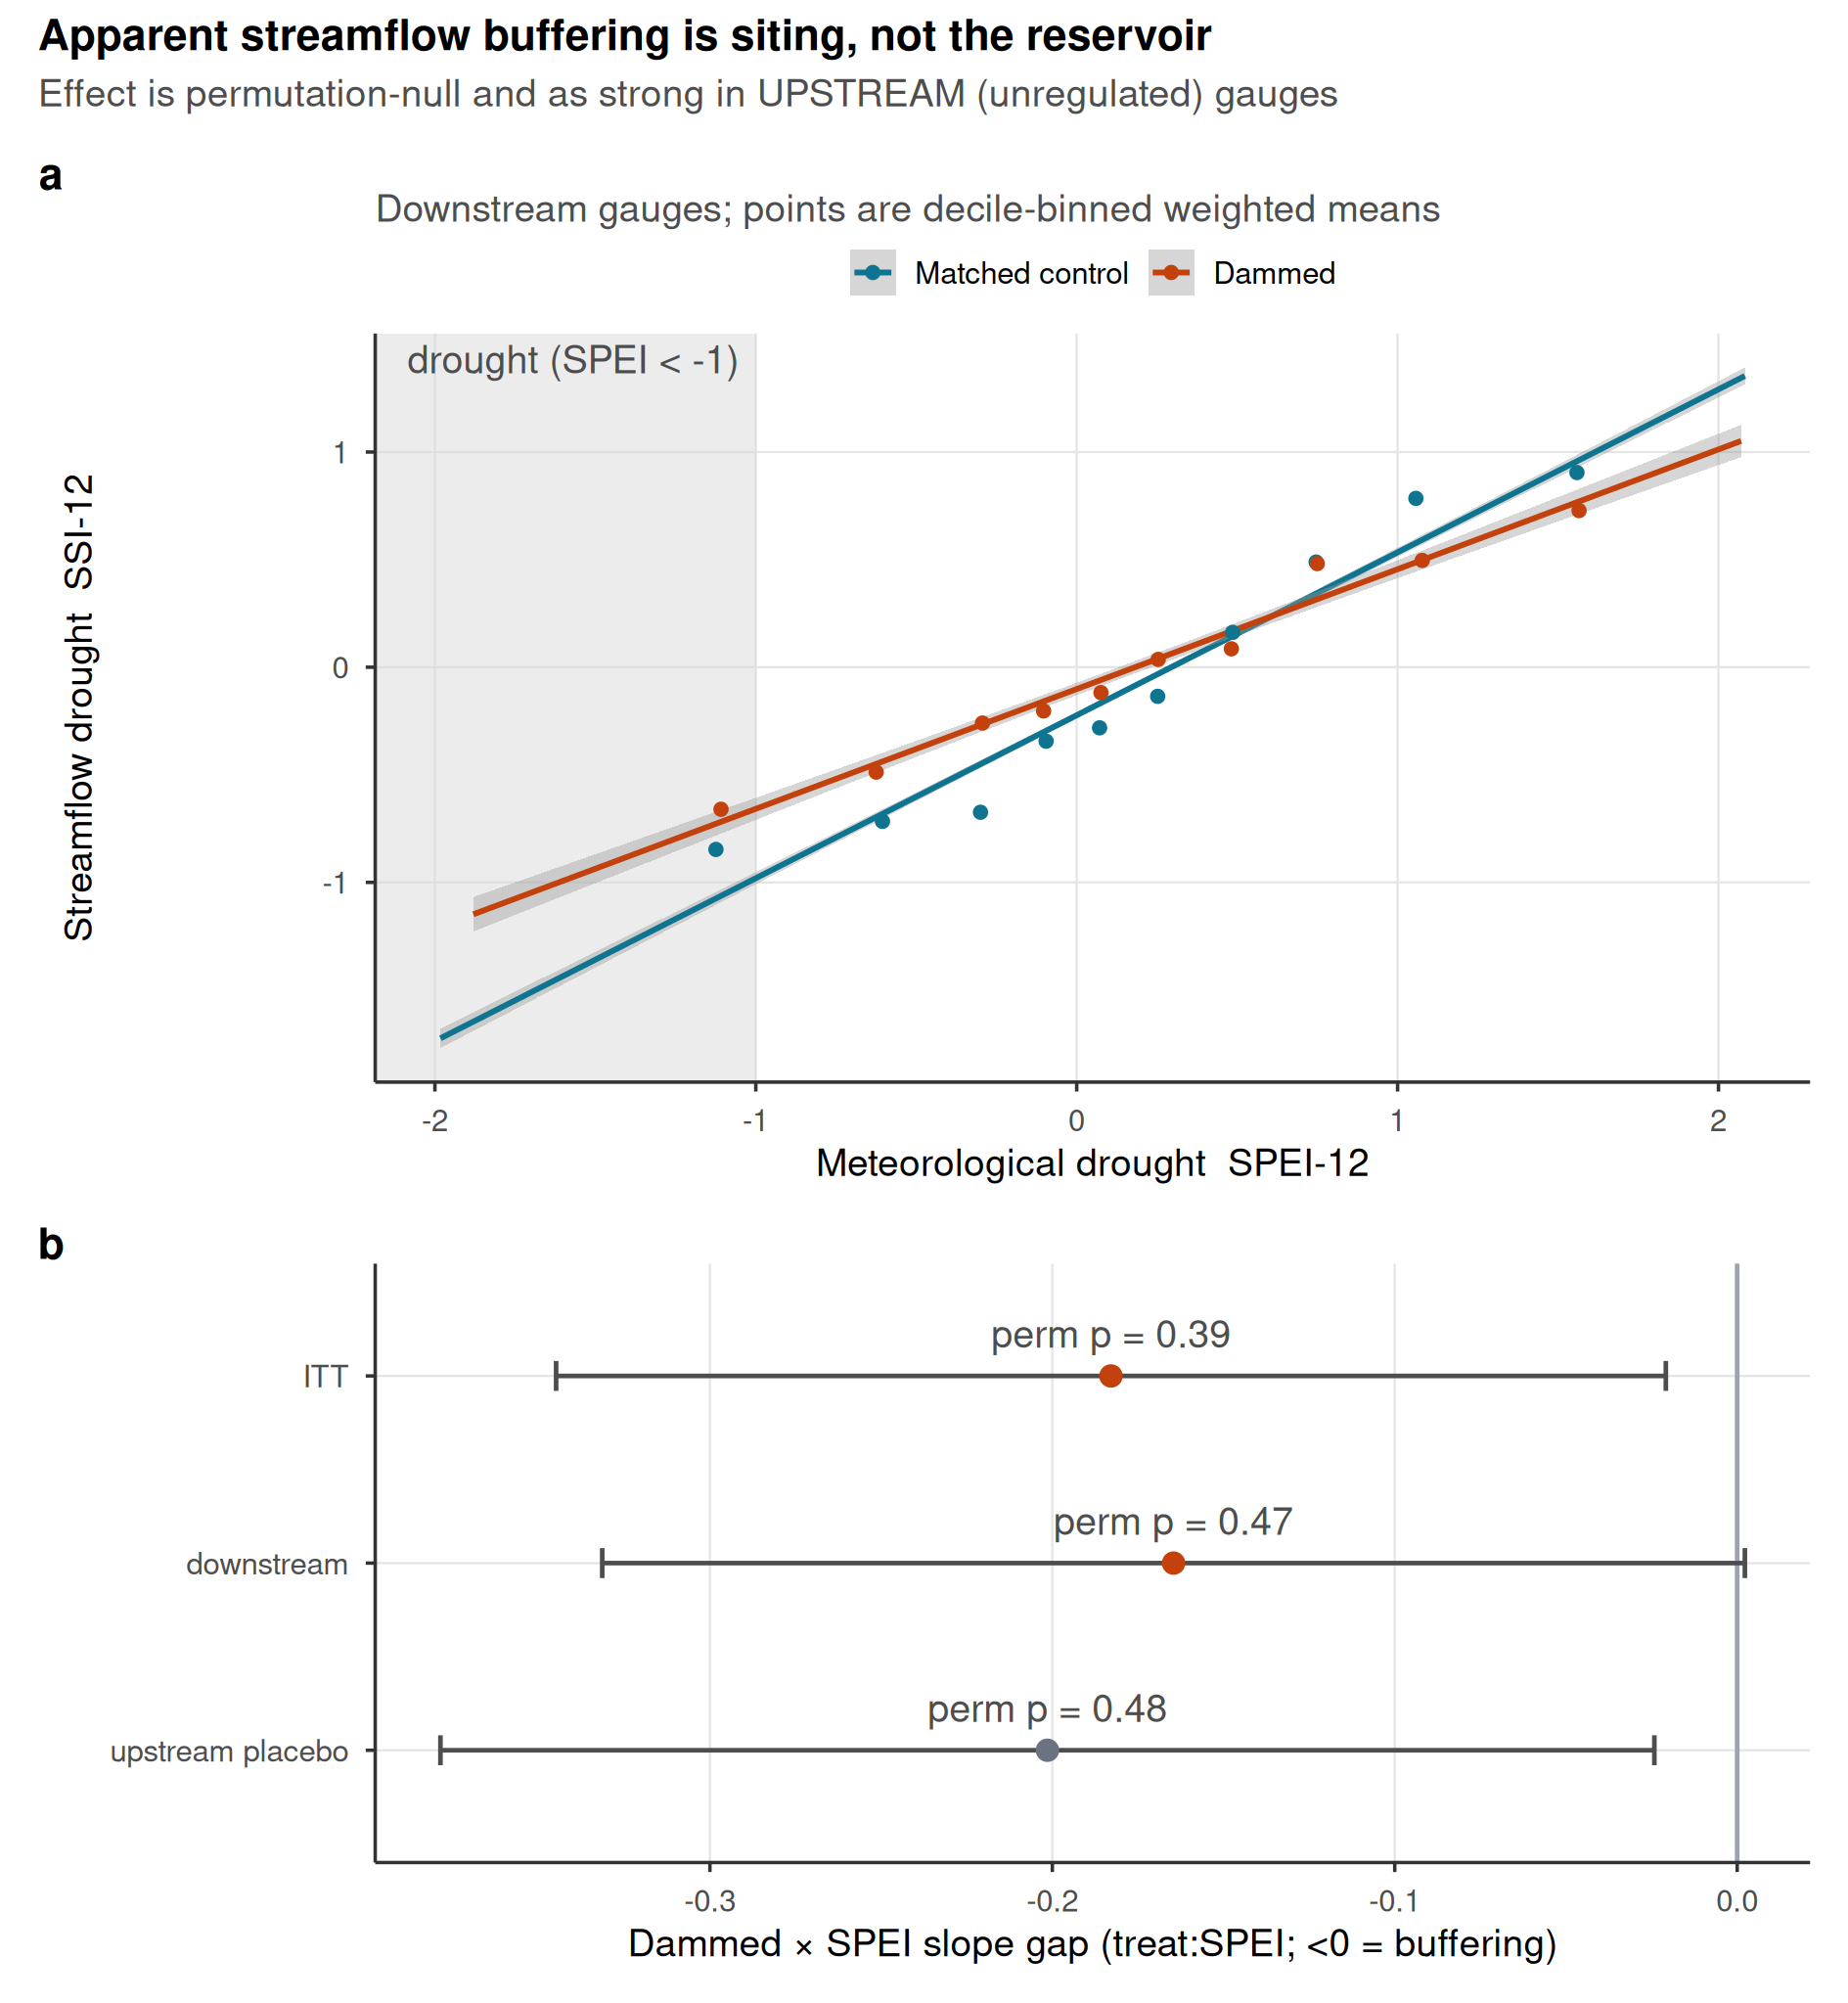
\includegraphics[keepaspectratio]{../../results/figures/fig_streamflow.png}}

}

\caption{\label{fig-streamflow}Streamflow buffering is reservoir siting,
not regulation. (a) SPEI-12 to SSI-12 transmission for dammed versus
matched-control basins (downstream gauges); lines are weighted
least-squares fits and shaded bands are 95\% confidence intervals;
dammed basins show a flatter slope, the apparent buffering. (b)
Differential slope (treat:SPEI; \textless0 = buffering) for
intent-to-treat, downstream-only, and the upstream-only placebo;
horizontal bars are 95\% confidence intervals (estimate +/- 1.96
cluster-robust SE), annotated with randomization-inference p-values. All
are permutation-null, and the upstream placebo (above-dam, unregulated)
is as strong as downstream, so the attenuation is siting/aridity, not
the dam.}

\end{figure}%

\subsection{No reservoir effect survives across any operational
pathway}\label{sec-bounding}

The same answer holds across the other pathways
(Figure~\ref{fig-forest}, Table~\ref{tbl-main}). Each effect is the
differential response of dammed and matched-control basins to the same
deficit, each estimate scaled by its own standard error, so a value
inside \(\pm 2\) is indistinguishable from no effect. Every estimate
that carries evidential weight brackets zero: cross-sectional
cropland-area expansion (\(-0.69\) ha km\textsuperscript{-2}, 95\% CI
\([-2.4, 1.1]\)) and its forcing-conditioned slope gap
(\(p_{\text{perm}} = 0.91\)). The evapotranspiration pathway is
relegated to the Supplementary Information: whole-basin ET is confounded
by barren-land aridity with failed pre-trends, and the post-hoc orchard
stratum relies on MODIS (Moderate Resolution Imaging Spectroradiometer)
MOD16 product, whose documented bias toward zero over irrigated land, a
product property identified independently of our results, disqualifies
its null (Supplementary Table S21, Fig. S7).

The null is informative but its power is concentrated in the streamflow
pathway. With about 21 dammed clusters the design cannot claim exact
equivalence to zero but rules out buffering above 46 to 59\% of
baseline, and a positive control confirms it: injected buffering is
recovered one-to-one and detected beyond that threshold (Methods;
Supplementary Fig. S2 and Tables S1, S3). Of the remaining pathways,
only the streamflow null excludes material effects at operationally
relevant magnitudes. The cropland and evapotranspiration designs are far
weaker, with minimum detectable effects orders of magnitude above
baseline (7,330\% and 237\% of baseline, respectively; Supplementary
Table S2); their nulls corroborate rather than independently establish
the absence of an effect. The water-rights count is comfortably null
under all inference frameworks (\(p_{\text{perm}} \geq 0.42\)), while
the winsorized volume is a more nuanced result discussed below.

\begingroup\fontsize{6}{8}\selectfont

\begin{longtable}[t]{lllrlll}

\caption{\label{tbl-main}Reservoir-effect estimates across estimators.
Cross-sectional doubly-robust matched ATTs (including the water-rights
induced-demand test) and forcing-interacted DiD slope gaps (treat:SPEI).
The DiD row and water-rights accrual are judged by
randomization-inference p-values (p), the design's primary inference at
\textasciitilde21 clusters; cluster-robust CIs are shown for
completeness and over-reject here. A positive estimate would indicate
induced-demand vulnerability; a negative one, operational buffering.
Evapotranspiration outcomes are relegated to the Supplementary
Information (Table S21, Fig. S7): whole-basin ET is confounded by
barren-land aridity with failed pre-trends, and the orchard rows rely on
MOD16, whose documented underestimation over irrigated land biases them
toward zero.}

\tabularnewline

\toprule
Group & Outcome & Estimand & Estimate & 95\% CI & p & Verdict\\
\midrule
Cross-sectional matched ATT & Cropland-area expansion & ha km\textasciicircum{}-2 added & -0.687 & {}[-2.44, 1.06] & - & null\\
Cross-sectional matched ATT & Water-rights accrual & rights / 100 km\textasciicircum{}2 added & 20.036 & {}[4.02, 36] & 0.52 & null\\
Forcing-interacted DiD (slope-gap) & Cropland area & differential deficit->impact slope & 0.001 & {}[-0.00344, 0.00493] & 0.91 & null\\
\bottomrule

\end{longtable}

\endgroup{}

\begin{figure}

\centering{

\pandocbounded{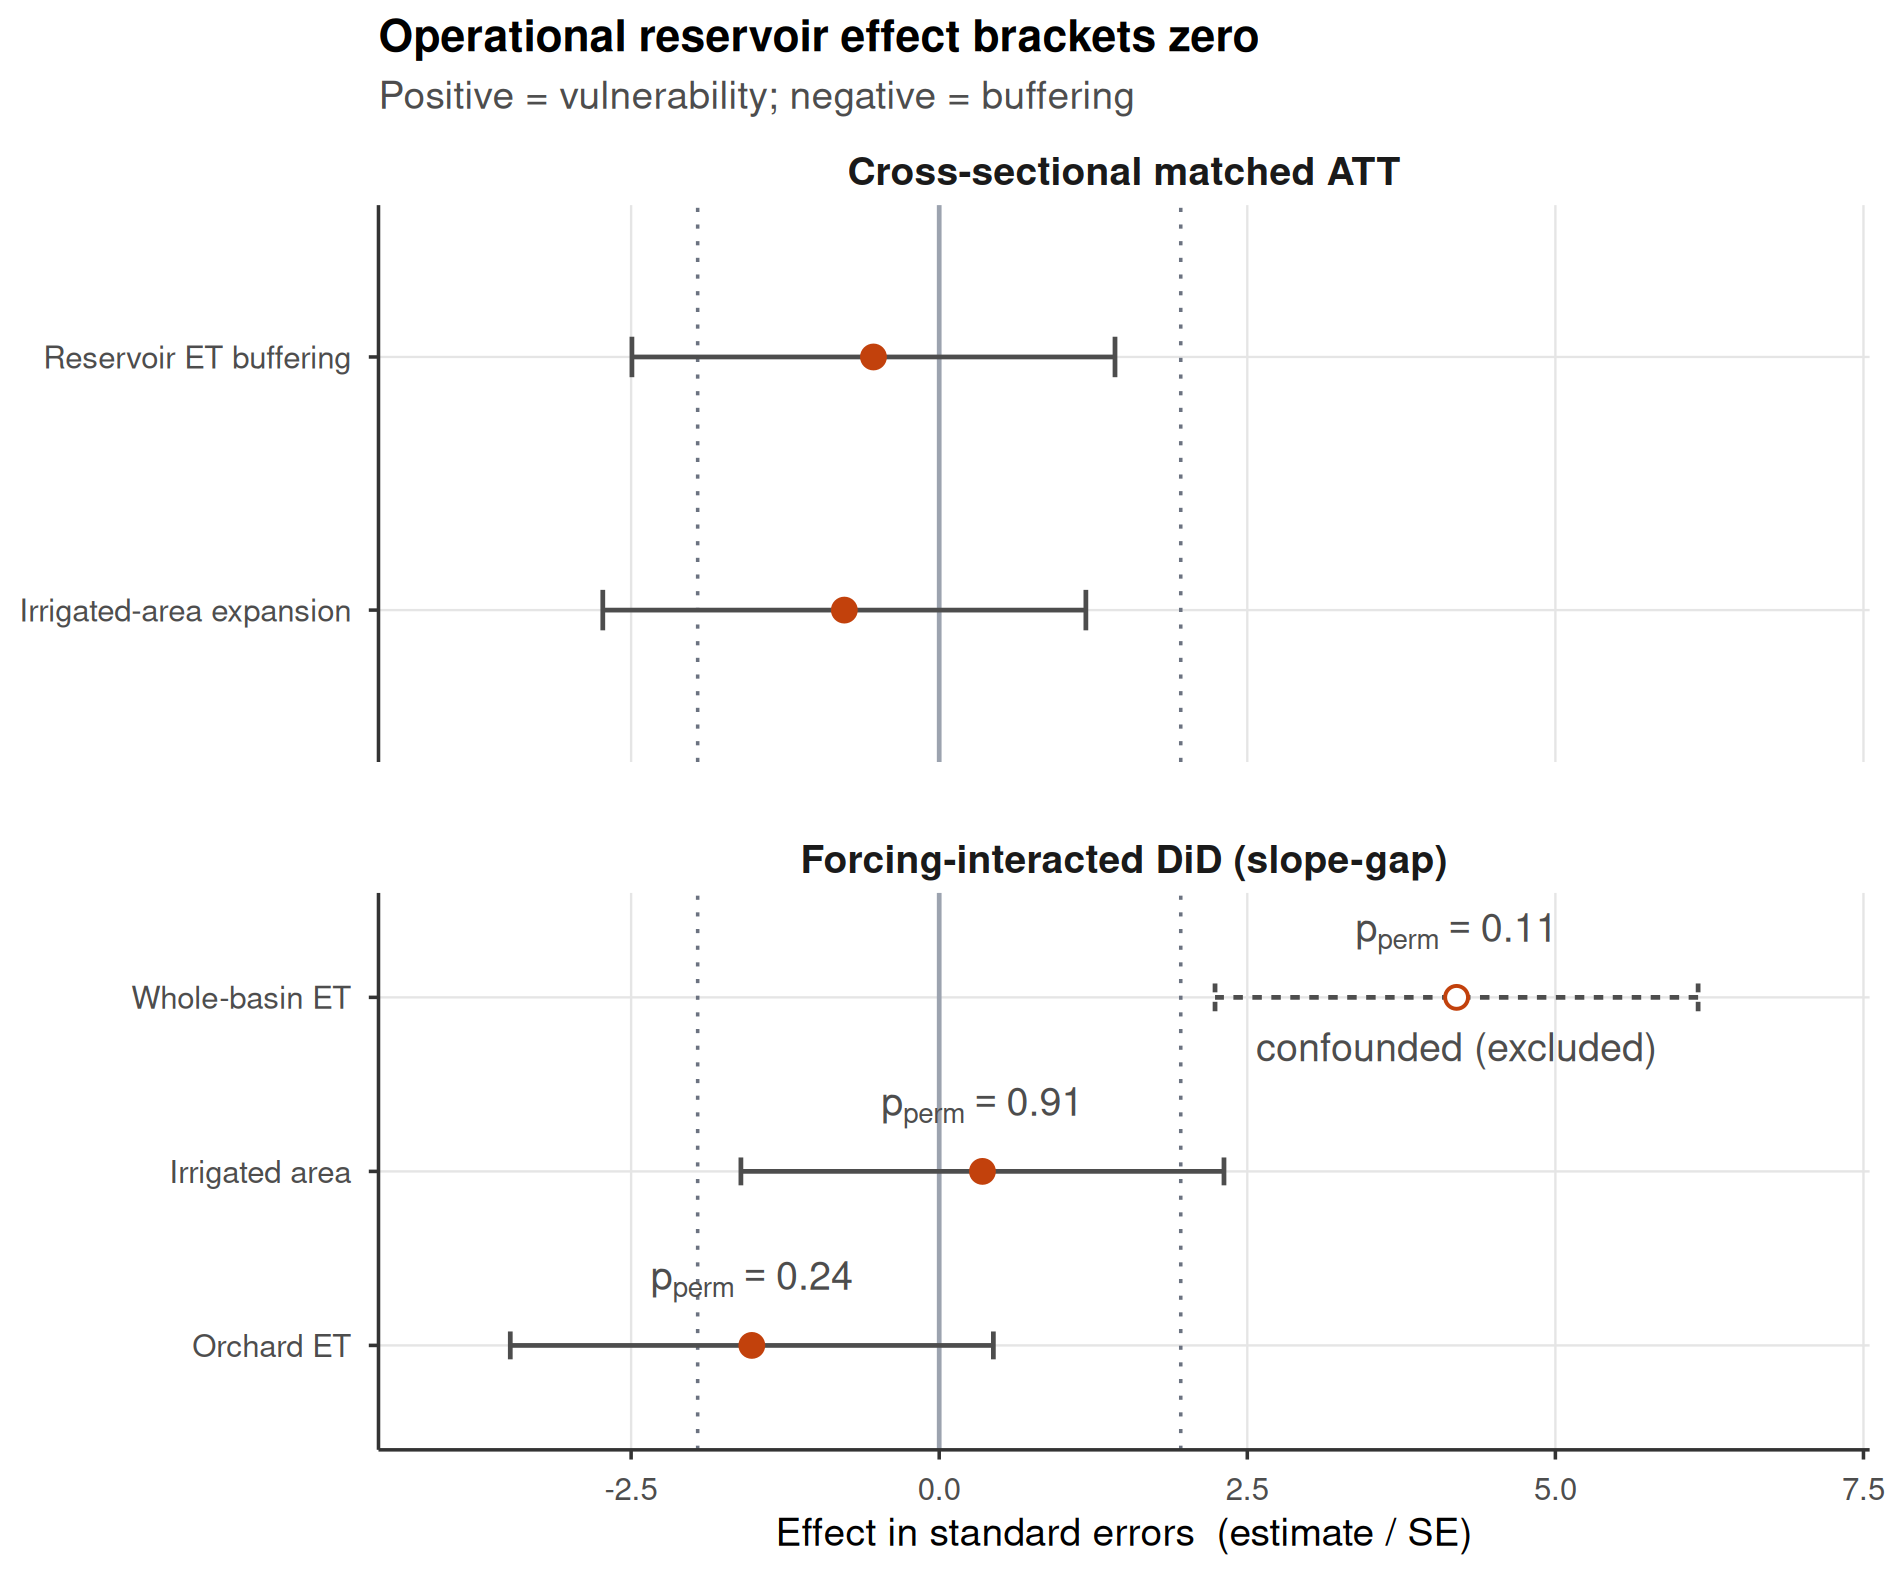
\includegraphics[keepaspectratio]{../../results/figures/fig_convergent_null.png}}

}

\caption{\label{fig-forest}Dammed-versus-control effect across the
estimators, each expressed uniformly in its own standard errors
(estimate divided by its SE) so the axis metric is identical for every
row; an estimate inside +/-2 is indistinguishable from no effect. Rows
are grouped by inference regime: cross-sectional matched ATTs (top) and
forcing-interacted DiD slope gaps (bottom). Bars span +/-1.96 SE (the
95\% reference interval) and dotted lines mark +/-1.96; a positive
effect would indicate induced-demand vulnerability, a negative one
operational buffering. Rows judged by randomization inference are
annotated with their p (the design's valid inference at
\textasciitilde21 clusters, since the +/-1.96 SE guides over-reject
there). Under that valid inference every estimate brackets zero.
Evapotranspiration outcomes are relegated to the Supplementary
Information (Table S21) as product-limited and confounded. Water-rights
accrual sits outside +/-1.96 by its naive standard error yet is null by
the design (p\_perm = 0.52; the apparent induced demand lies inside the
permutation null expected from the dammed basins' unbalanced aridity,
Supplementary Fig. S6).}

\end{figure}%

\subsection{Reservoirs mark prior vulnerability; no megadrought
divergence is
detected}\label{reservoirs-mark-prior-vulnerability-no-megadrought-divergence-is-detected}

Dammed basins carry the vulnerability reservoirs are blamed for
concentrating: about 4.5 times more cropland than matched controls
(10.8\% versus 2.4\% of basin area; Figure~\ref{fig-area}, panel a).
This gap is a \emph{siting} signature, stable across the 2000--2024
record. A dynamic event study finds the differential trend flat before
2010 (cluster-robust \(p = 0.65\), permutation \(p = 0.72\)) with no
post-2010 divergence detected (\(p = 0.81\); Figure~\ref{fig-area},
panel b). Both are bounded nulls, not confirmations of parallelism: the
pre-trend test detects only divergence accumulating to about half the
control cropland level by 2009 (the observed trend is a seventh of
that), and the permutation envelope widens after 2015, so the late panel
cannot rule out substantial divergence (Supplementary Table S14). The
null is metric-invariant: on log cropland share the slope gap is
likewise permutation-null (\(p = 0.37\); Supplementary Table S20).
Reservoirs mark where cropland already was; within these bounds they
neither expanded it nor changed its drought response.

The same holds for the most direct demand measure. In the Chilean Water
Directorate (DGA) registry of consumptive water rights, dammed basins
appear to accrue rights faster than controls, on both the outlier-robust
count (\(+20\) per 100 km²; Figure~\ref{fig-forest},
Table~\ref{tbl-main}) and the winsorized volume (\(+2.5\) l/s per km²;
Supplementary Fig. S6), each with an analytic interval excluding zero.
This is the naive-analysis trap the design catches: dammed basins are
more arid, arid basins carry denser water-rights activity, and the
imbalance drives the gap. The count does not survive randomization
inference (\(p_{\text{perm}} = 0.52\); Supplementary Fig. S6) and
remains null under a fully non-parametric match on the aridity-overlap
subset (\(p_{\text{perm}} = 0.42\); Supplementary Table S7). The
winsorized volume is more delicate: stable across thresholds and
physically validated (Supplementary Table S8), its overlap-subset
permutation p falls to \(0.005\), but the residuals are spatially
autocorrelated (Supplementary Table S9) and under the governing
cuenca-block permutation it is not significant
(\(p_{\text{perm}} = 0.077\), cuenca-clustered interval
\([-0.3, 4.1]\)). Ranked raw, uncapped volumes give the same verdict:
the design rank contrast is null under cuenca-block permutation
(\(p = 0.15\); Supplementary Table S18). The water-rights evidence is
therefore not uniformly null: the count is cleanly so under all
frameworks, the ranked raw volumes are null under spatial inference, and
the winsorized volume sits closer to the boundary, with a unit-level
signal (\(p = 0.005\)) that the spatial structure partially explains but
does not fully erase (cuenca-block \(p = 0.077\)). The gap between naive
and spatial inference flags the spatial concentration of large
consumptive rights in dammed cuencas, a pattern the design can bound but
whose attribution to siting versus reservoir-induced demand it cannot
fully resolve at this spatial grain. No induced demand is robustly
attributable to the reservoir once siting and spatial structure are
accounted for, but the volume signal warrants further investigation with
parcel-level consumption data.

\begin{figure}

\centering{

\pandocbounded{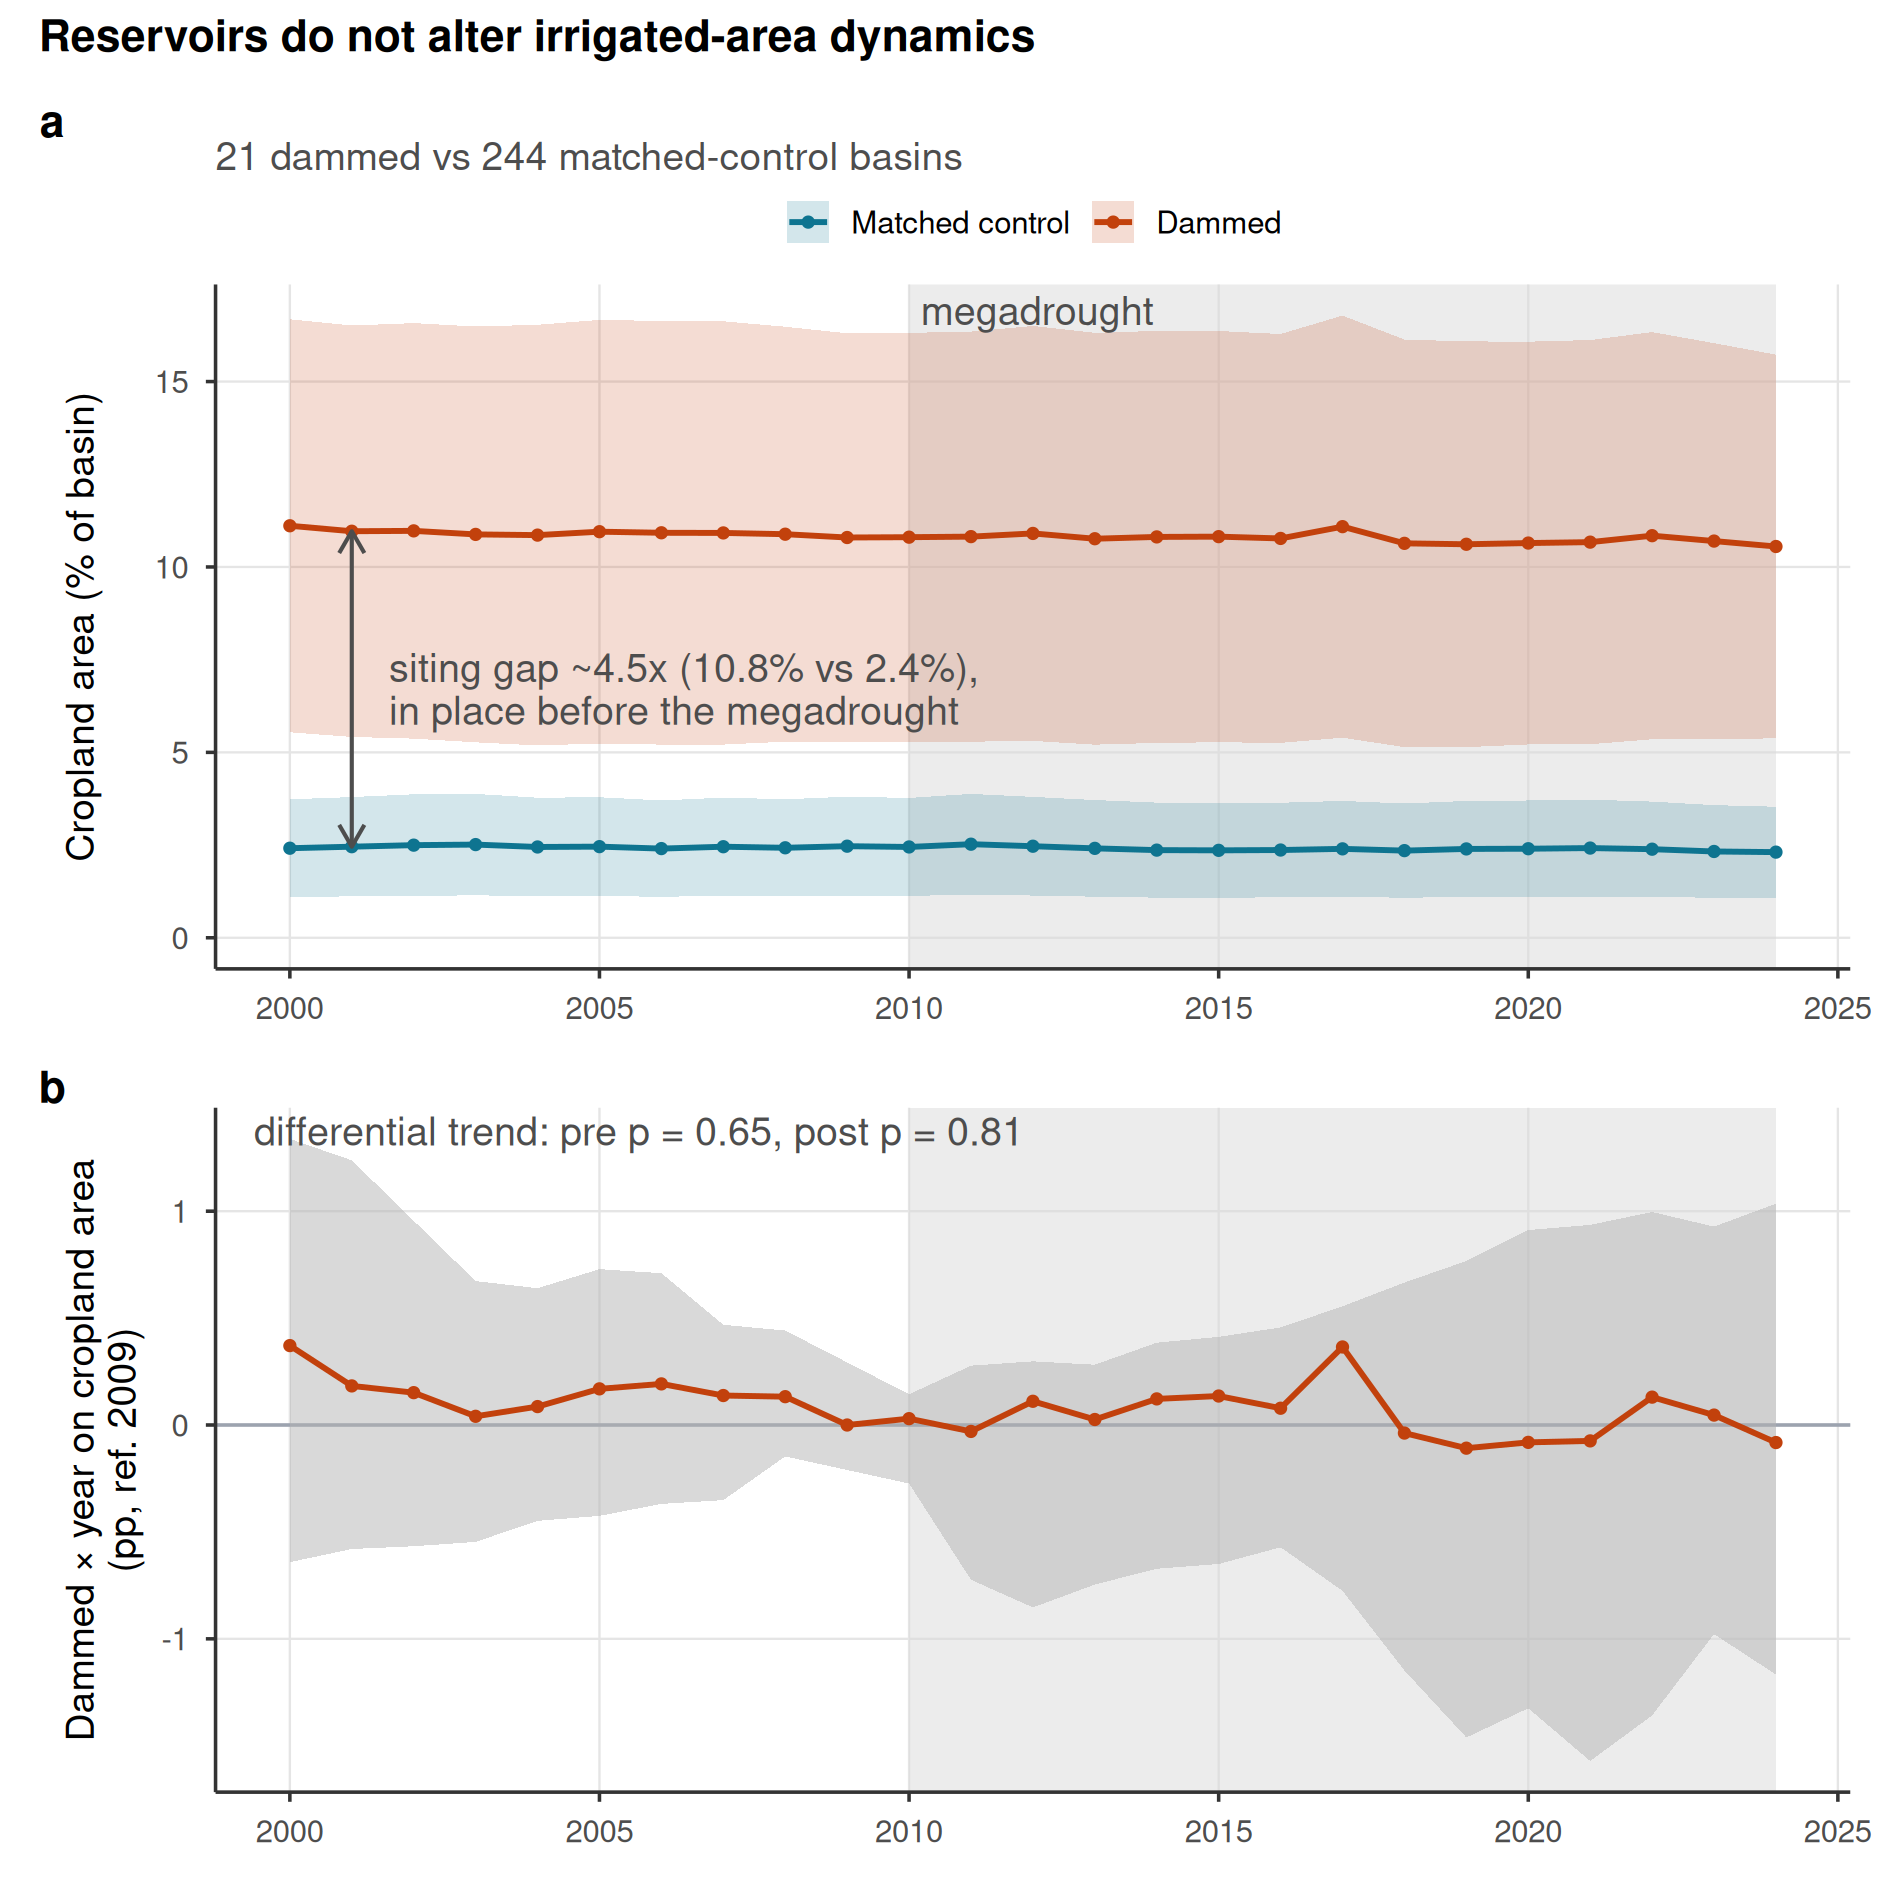
\includegraphics[keepaspectratio]{../../results/figures/fig_area_did.png}}

}

\caption{\label{fig-area}Observed cropland-area dynamics in dammed
versus matched-control basins (21 dammed, 244 controls). (a)
Entropy-balancing-weighted mean cropland area (\% of basin, MapBiomas
class 18) with 95\% bands (weighted mean +/- 1.96 SE across basins); the
y-axis is anchored at zero. Dammed basins hold \textasciitilde4.5x more
cropland (10.8\% vs 2.4\% of basin area) but the trajectories evolve in
parallel. (b) Dynamic event study (dammed x year, reference 2009): the
grey band is the 95\% randomization-inference null envelope (2.5th to
97.5th percentile of the dammed x year coefficients under treatment
permutation within Köppen x aridity strata); coefficients inside the
band are indistinguishable from no divergence, and cluster-robust
intervals are omitted as anti-conservative at \textasciitilde21 treated
clusters. The differential pre-trend is flat (pre-2010 trend-slope
cluster-robust p = 0.65, permutation p = 0.72) and no post-2010
divergence is detected (post p = 0.81); a linear trend-slope test is
used because the joint event-study Wald over-rejects at
\textasciitilde21 treated clusters. The null envelope widens after 2015,
reflecting declining power in the later panel, so the flat post-2015
trajectory is a bounded null: divergence smaller than the envelope
cannot be ruled out. The 2010-2024 megadrought is shaded in both
panels.}

\end{figure}%

\subsection{Storage falls; a change in refill amplitude cannot be
resolved}\label{storage-falls-a-change-in-refill-amplitude-cannot-be-resolved}

If the streamflow pathway excludes material operational buffering and
the demand-side pathways are consistent with no amplification at their
respective detection limits, what matters is how much water there is to
store (Figure~\ref{fig-storage}). Over 2005--2024 the storage band
drifts downward in step: peak storage falls by 1.3 percentage points of
capacity per year (\(p = 0.013\)) and the trough almost identically
(\(1.2\) pp yr\textsuperscript{-1}, \(p < 10^{-4}\)), while the seasonal
amplitude shows no detectable trend (\(-0.06\) pp
yr\textsuperscript{-1}, \(p = 0.91\); Supplementary Table S5). That
amplitude interval is wide: whether refill amplitude, the buffering
capacity, has degraded cannot be determined, and we draw no conclusion
about it. The decline is a level shift at the megadrought onset rather
than a secular line (peak 87\% of capacity before 2010, 67\% after;
trough 40\% to 25\%; Supplementary Table S5). That decline is
commensurate with the supply reduction measured independently in the
matched controls: unregulated control streamflow fell about 2.9\% per
year over 2005--2020 (dammed 3.4\%), consistent with documented
megadrought runoff deficits (R. D. Garreaud et al. 2017;
Alvarez-Garreton et al. 2021) and comparable to the \textasciitilde1.4\%
per year decline in peak storage. Storage is a mass balance, so the band
alone cannot separate falling inflows from sustained releases; the
supply reading rests on that independent streamflow decline. Our direct
demand outcomes point the same way: neither cropland area nor
water-rights allocation shows expansion (Figure~\ref{fig-area},
Table~\ref{tbl-main}; Supplementary Fig. S6) (Li et al. 2023; Z. Wang et
al. 2024).

\begin{figure}

\centering{

\pandocbounded{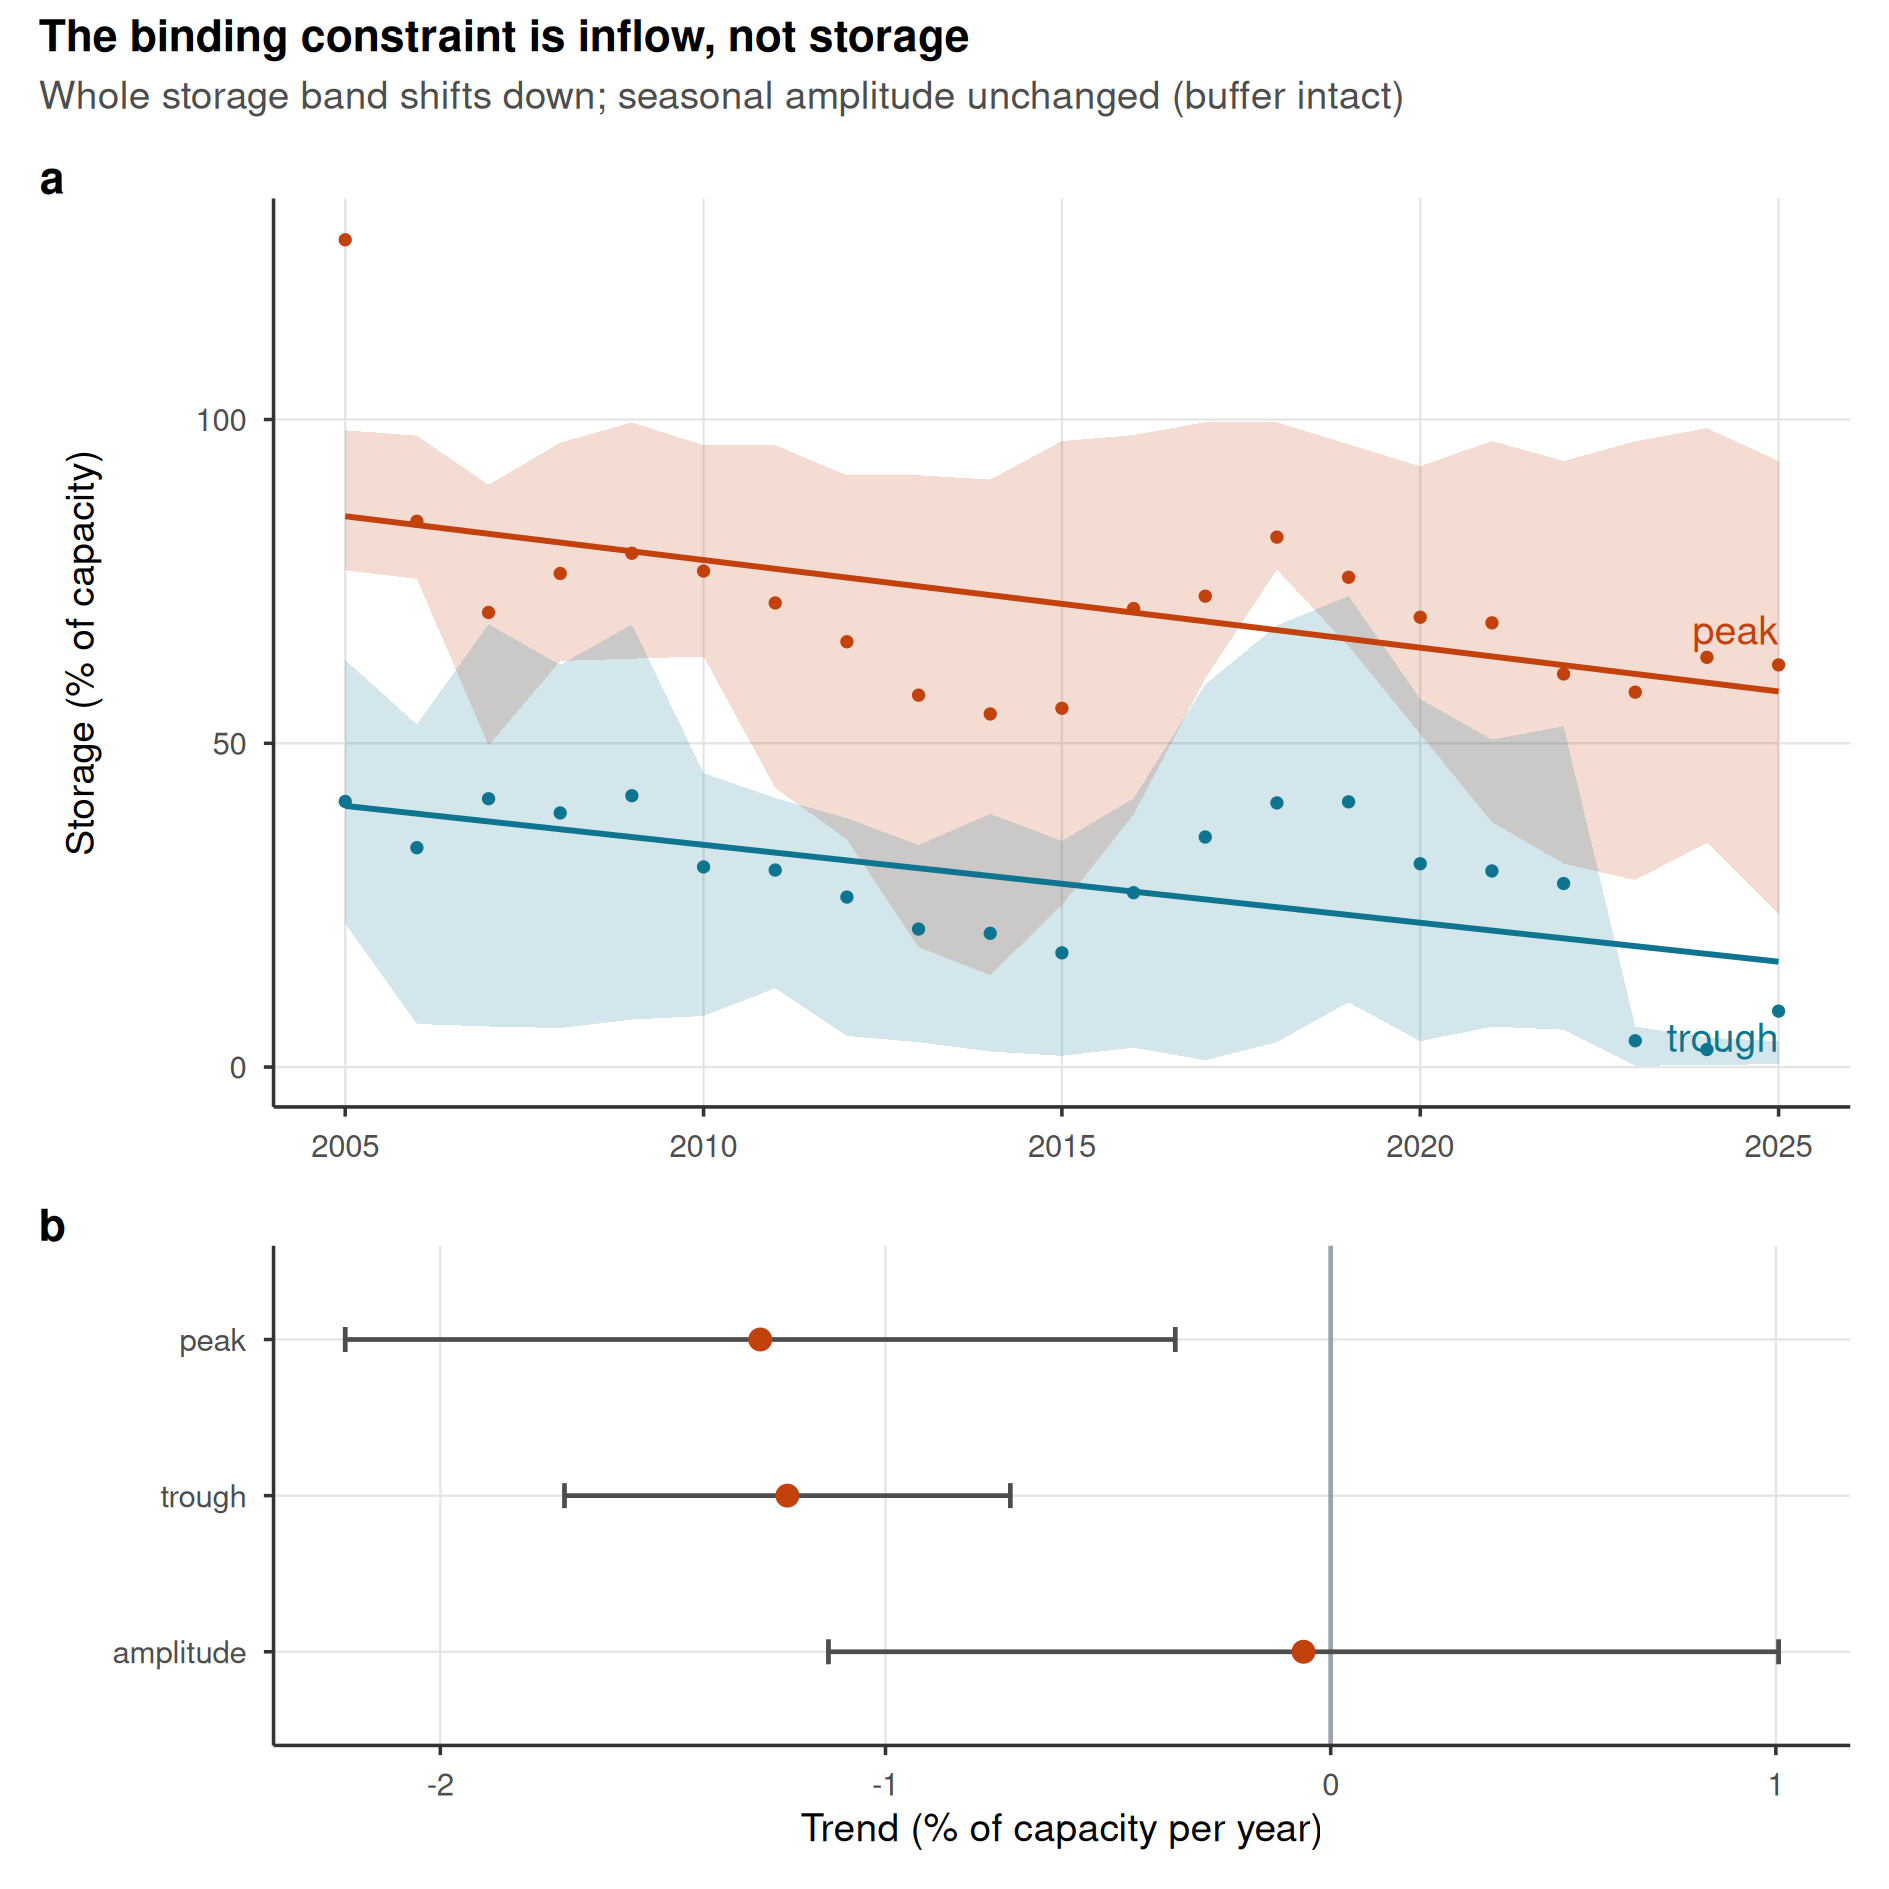
\includegraphics[keepaspectratio]{../../results/figures/fig_storage_band.png}}

}

\caption{\label{fig-storage}Reservoir storage declines; a change in
seasonal refill amplitude cannot be resolved. (a) Cross-reservoir annual
storage band: realized median peak and trough percent-of-capacity (solid
lines) with interquartile ribbons across reservoirs, and the peak-trough
amplitude (grey dashed). Medians are used because a few reservoirs
report storage above nominal capacity (dotted 100\% line); the whole
band drifts down over 2005-2024 while the amplitude does not narrow.
Central lines are the realized medians, not linear fits; the net trend
is quantified in (b). (b) Per-year trend slope of peak, trough, and
amplitude (reservoir fixed effects); error bars are 95\% confidence
intervals (estimate +/- 1.96 cluster-robust SE): peak and trough both
decline while the amplitude trend is not distinguishable from zero (a
wide interval, so statistically unchanged rather than proven constant),
consistent with a supply-side level decline rather than refill/buffer
degradation. Descriptive: pooled within-reservoir trend, no control
group.}

\end{figure}%

\section{Discussion}\label{discussion}

Across a matched national design, multiple estimators, and a
within-basin falsification test, the apparent drought buffering
attributed to reservoirs is a measurable siting confound. The upstream
placebo is the decisive evidence: a regulation effect must appear only
below the dam; it does not, and what remains is the aridity gradient.
Dammed basins hold about 4.5 times more cropland than matched controls,
but that gap is fixed across the record, with parallel pre-trends and no
detected megadrought divergence. One reading fits: reservoirs mark where
water-dependent vulnerability already concentrated rather than make it.
This is a finding, not a failure of power: the apparent effect has an
identified cause and the positive control shows the design detects
buffering when it is present.

The corollary is transferable: dammed-versus-undammed or before-after
contrasts inherit the full siting confound (López‐Moreno et al. 2009; Wu
et al. 2017; Schilstra et al. 2024; Lee, Kang, and Kim 2026). The
upstream placebo ports to regulated rivers with gauges above and below a
dam, most directly to short, steep catchments like Chile's; in large
low-gradient basins, floodplain storage and transmission losses would
blur the contrast; porting it would need routing-corrected lags or
naturalized-flow counterfactuals.

If the streamflow pathway excludes material operational buffering at
multi-year scale and the demand-side outcomes are consistent with no
amplification at their respective detection limits, what matters is the
water available to store. The storage band steps down at the megadrought
onset, peak and trough together, while the amplitude trend is too
imprecise to determine whether buffering capacity degraded. The powered
result is the level decline, the expected mass-balance outcome of
persistent inflow deficits; descriptive and confounded with management
change, it supports no causal attribution but matches the independent
decline in unregulated control streamflow. Read against Chile's
structural aridification (Zambrano et al. 2025; R. D. Garreaud et al.
2017; Alvarez-Garreton et al. 2021), accelerating Andean warming and
snow loss now cutting into the snow-fed streamflow these basins depend
on (Kim, Rajaram, and Lakshmi 2025), and the global pattern of
reservoirs failing to refill (Z. Wang et al. 2024; Li et al. 2023), the
binding constraint is shifting toward supply.

These findings give the contested socio-hydrological \emph{reservoir
effect} and \emph{supply-demand cycle} (Di Baldassarre et al. 2018;
Kellner 2021) a credibly identified test, and find the protective
function over-attributed to storage. Because treatment is
time-invariant, we test the spatial imprint of these feedbacks, not the
longitudinal loop. The 4.5-fold cropland gap could be the equilibrated
legacy of demand induced at construction, so our null covers the
megadrought era; historical induced demand is testable only with
staggered commissioning. And the record opens in the scarcity phase,
after any expansion under perceived abundance, so it bounds drought-era
expansion, not the cycle as a whole. Within scope the nulls refine the
theory: the cycle leaves no operational imprint during drought, so its
mechanisms likely act through siting and construction rather than
operation, a distinction current models omit. How far the demand-side
null travels depends on governance: the siting lesson holds wherever
dams are placed non-randomly; prior appropriation, which forfeits unused
rights, may amplify induced demand while adaptive allocation curtails
it. Whether the null is general or the mark of a fully allocated market
we cannot adjudicate: rights kept accruing in dammed basins, but systems
with water still unallocated could express an induced demand that ours
cannot. The upstream placebo itself ports more broadly. Short, steep
catchments with gauges above and below dams are common across the
world's regulated mountain rivers: the California Coast Ranges and
Sierra Nevada, the Spanish Sierra Nevada and Pyrenees, the Italian
Apennines and Alps, the African Rift, and the Andean cordillera beyond
Chile. In large low-gradient basins, the Murray-Darling, the Colorado
below Lake Mead, or the Indus plains, floodplain storage and
transmission losses would blur the above/below contrast and
routing-corrected lags or naturalized-flow counterfactuals would be
needed. The placebo method is therefore not universal, but its scope
conditions are explicit and its required data, paired gauges above and
below dams, exist across much of the world's irrigated mountain-front
hydrology.

Chile's 1981 Water Code makes water-use rights perpetual private
property, so the reflexive response has been supply-side, new dams and
inter-basin transfers (Barría et al. 2021; R. Garreaud et al. 2025); the
2022 reform moves toward the adaptive allocation our results argue for
(Macpherson et al. 2023) but postdates our window. Under structural
aridification, building more storage is a supply-blind response to a
supply problem: the buffering dams provide is a property of where they
sit, not of what they do (Ho et al. 2017). Adaptation must shift toward
demand management, reallocation and managed aquifer recharge (Grafton et
al. 2018; Scanlon et al. 2023; Rivera-Vidal et al. 2025).

Several limitations bound these conclusions, each quantified in the
Supplementary Information. The result is a bounded null: the design
excludes streamflow buffering above 46 to 59\% of baseline, demand-side
outcomes are far less powered and the pre-trend test power-limited
(Supplementary Tables S2, S14), so causal weight rests on the placebo,
demand nulls corroborating; all survive the hard-balanced match
(Supplementary Table S17). The registry measures paper rights, not wet
water: Chilean basins are widely over-allocated and granted rights can
sit unused or hoarded (Barría et al. 2021; Reade Malagueño and D'Odorico
2024), so under drought, when physical availability binds, the accrual
we test is an entitlement response that non-use could dampen; cropland
is the physical check. Both metrics also miss intensification within an
unchanged footprint; central Chile's documented shift toward thirsty
export fruit (Reade Malagueño and D'Odorico 2024) is exactly such a
transition, invisible to both; a consumption-grade test awaits thermal
ET or crop-transition maps. Groundwater substitution is bounded, dammed
and control water tables falling at indistinguishable rates across 213
DGA wells despite severe regional drawdown (Taucare et al. 2024);
monitored wells need not sample the orchard footprints where pumping
concentrates, so unmonitored drawdown could sustain a historically
reservoir-induced footprint (Supplementary Table S10). In that reading
the reservoir effect is not absent but displaced to the aquifer, a
construction-era legacy persisting on a pool the design cannot see; the
well bound and flat cropland trajectories argue against substitution at
scale but do not close the pathway. The snowmelt confound, acute in
these snow-fed Andean basins (Ayala et al. 2025; Götte and Brunner
2024), is tested on the differential estimand and excluded across four
specifications (Supplementary Table S12). The geomorphic check leaves
the placebo unchanged, though 2.5 km relief cannot resolve aquifer
storage itself, a residual caveat (Supplementary Table S22). The placebo
also spans land-cover and abstraction contrasts, downstream valleys more
cultivated, upstream reaches carrying unrecorded diversions; gauge fixed
effects absorb these level differences, and drought-intensified upstream
abstraction would steepen upstream transmission, working against the
observed upstream attenuation, not producing it. Administrative closure
cannot force the demand null: treated basins entered the drought with
higher allocated stock yet accrued rights 2.7 times faster, and parallel
control cropland contradicts collapse prevention (Supplementary Table
S15). No matched pair shares a watershed; outbound transfers would
shrink the gap and imports would mimic downstream-specific buffering,
which is absent (Supplementary Table S15); irrigation-only restriction
leaves the result unchanged (Supplementary Table S11). MOD16's bias
toward the null excludes the ET pathway from evidence (Supplementary
Table S21); the demand conclusion rests on cropland and the registry,
with thermal ET as future work. Finally, the 12-month accumulation
targets multi-year vulnerability, not the sub-seasonal buffering
reservoirs also provide, which we neither test nor dispute. The fleet is
partly seasonal by design, the median treated reservoir storing 0.3
years of downstream flow, yet seven of 17 hold at least half a year,
four exceed a year, and none empties seasonally (Supplementary Table
S23): carryover was physically available, so its absence in outcomes is
not a design tautology. Two extensions can test what our window cannot:
a staggered event study of cropland around historical commissioning
would probe construction-phase induced demand; a rule-curve
quasi-experiment on release records, once public, would isolate
operation.

At the multi-year timescale of structural aridification, then, the
design detects neither operational buffering nor megadrought-era demand
expansion beyond the siting legacy: the apparent buffering is a
statistical shadow of where dams sit, not of what they do, while the
water available to store declines. The nulls are bounds, not zeros;
effects inside them can be volumetrically material (Supplementary Table
S16). But under structural aridification with no operational buffering
at the multi-year scale, building more storage is a supply-blind
response to a supply problem. Chile is currently evaluating at least 26
new reservoir sites to expand storage, while its agricultural water
demand continues to grow under perpetual private water rights that the
2022 Water Code reform only begins to address (Macpherson et al. 2023).
The alternative is not theoretical: demand reallocation through active
water markets, irrigation efficiency, managed aquifer recharge, and crop
transitions toward lower water footprints are available now and do not
depend on rainfall (Grafton et al. 2018; Scanlon et al. 2023;
Rivera-Vidal et al. 2025). Resilience to a falling supply ceiling will
come from confronting demand and allocation, not from more impoundments.

\section{Methods}\label{methods}

\subsection{Study area and design}\label{study-area-and-design}

We study continental Chile (≈18--44° S), a strong north--south aridity
gradient spanning hyper-arid, Mediterranean, and humid-temperate
climates, over 2005--2024, the window in which reservoir storage,
meteorological forcing, and satellite outcomes jointly exist. The design
is a matched comparison of dammed versus undammed sub-watersheds, with
reservoir presence treated as a basin-level intervention. Because the
reservoirs in most treated basins (18 of the 24) were commissioned
before the storage record begins, treatment is effectively
time-invariant over the window and a staggered-adoption (commissioning)
event study is infeasible; identification therefore rests on a matched
cross-section combined with conditioning on meteorological forcing
rather than on calendar time.

The central estimand is the operational effect of a reservoir on drought
outcomes \emph{conditional on the covariates that govern where
reservoirs are sited}, that is, whether dammed basins respond to the
same drought forcing differently from hydroclimatically comparable
undammed basins. This isolates reservoir \emph{operation} from reservoir
\emph{siting} (Di Baldassarre et al. 2018).

\subsection{Spatial units and treatment
assignment}\label{spatial-units-and-treatment-assignment}

The analysis grain is the DGA sub-watershed (467 units), chosen over the
coarser watershed grain (101 units) for power and common support,
reservoirs sit in Chile's largest main-stem basins, and the finer grain
supplies far more controls inside the treated size range (detailed in
the archived analysis repository). A sub-watershed is treated if it
contains ≥1 of the 26 monitored reservoirs by point-in-polygon
assignment, giving 24 treated units (two reservoirs share a
sub-watershed). After entropy balancing, three high-Andes treated units
fall outside local elevation common support, leaving 21 treated basins
in all analyses; the progression from 26 reservoirs to 24 treated
sub-watersheds to 21 retained treated units is fixed across every
estimator and table. The reservoirs are predominantly irrigation (20 of
26; three hydropower, two potable supply, one mixed), so the treated set
is dominated by the use type built to buffer agricultural drought, and
the headline streamflow result is unchanged when restricted to
irrigation-only treated basins (Supplementary Table S11). An untreated
sub-watershed that lies within a watershed containing a reservoir is
flagged as contaminated (it shares the regulated main stem and is not a
clean counterfactual) and removed (45 units), leaving 398 clean
controls. This contamination rule defuses the most direct
downstream-spillover (SUTVA: Stable Unit Treatment Value Assumption)
violation; residual adjacency and shared-aquifer spillovers between
neighbouring sub-watersheds are carried as an identification caveat and
addressed with watershed-level checks: where spatial dependence is
present, inference is re-run with watershed-block permutation and
watershed-clustered intervals (Supplementary Table S9), and no matched
treated-control pair shares a watershed (Supplementary Table S15).

\subsection{Data}\label{data}

\textbf{Reservoir storage and treatment.} Monthly storage for 26
monitored reservoirs (the DGA record runs January 2005 to April 2026; we
analyse the complete calendar years 2005--2024) with a per-reservoir
capacity column (maximum level in hm³); storage and capacity share units
(hm³), so percent-of-capacity
(\texttt{100\ ×\ level\ /\ maximum\ level}) is the
cross-reservoir-comparable state variable. Static attributes
(commissioning year, use, size class) come from the national dam
registry.

\textbf{Meteorological forcing.} The Standardized
Precipitation-Evapotranspiration Index (SPEI) at a 12-month
accumulation, derived from Climate Hazards Center InfraRed Precipitation
version 3 (CHIRPS) and Climate Hazards Center InfraRed Temperature with
Stations (CHIRTS) and standardized on the 1991--2020 climatological
baseline (Sergio M. Vicente-Serrano, Beguería, and López-Moreno 2010),
is the primary exogenous dose; CHIRPS-derived standardized indices are
validated for Chilean drought monitoring, including ENSO-modulated
variability across the country (Zambrano et al. 2017; Meza 2013; Oertel,
Meza, and Gironás 2020). We use the 12-month accumulation because it
matches the annual, snowmelt-fed hydrological cycle of central Chile
(winter precipitation stored as snow and released through the growing
season) and so captures the inter-seasonal carryover that irrigation
reservoirs are built to bridge, at the scale at which multi-year
vulnerability (rather than sub-seasonal operation) is expressed. The
treatment estimates are insensitive to this choice: re- estimating the
forcing-conditioned effect with 6- and 24-month accumulations leaves it
materially unchanged (archived analysis code). By construction the
12-month window does not resolve short-term (1--3 month) operational
buffering, which reservoirs are documented to provide (Wu et al. 2017,
2018) and which we flag as a boundary of our conclusions (Discussion).
Conditioning on forcing (estimating effects on the deficit-to-impact
\emph{slope} rather than on levels) is how we break the collinearity
between the 2010-onset megadrought and the treatment clock.

\textbf{Hydrological drought.} Daily streamflow from the DGA network
(2000--2020), gathered by the CR2 (Center for Climate and Resilience
Research, https://cr2.cl) is aggregated to the Standardized Streamflow
Index at 12 months {[}SSI-12; Sergio M. Vicente-Serrano et al. (2012);
Lema et al. (2025){]}, the regulated-flow analogue of SPEI-12 and the
index in which meteorological deficits are re-expressed as hydrological
drought, a propagation that reservoir operation is known to modify by
lengthening and attenuating the transmitted signal (Van Loon 2015; W.
Wang et al. 2016), used as the outcome in the within-basin placebo
(below). Gauges are classified as upstream or downstream of each dam
from an SRTM digital elevation model. Because SSI standardizes each
gauge on its own, for regulated gauges post-dam, flow distribution, the
transmission slope tests distribution-relative propagation and would
divide out any dam-induced variance compression; we therefore
re-estimate every buffering model and the placebo on log 12-month mean
flow, a volumetric semi-elasticity (percent of flow per SPEI unit) that
no per-gauge normalization can compress, and test the compression
premise itself, the deseasonalized relative flow variability by gauge
class (Supplementary Table S19).

\textbf{Ecological and land-use outcomes.} (i) annual cropland area from
MapBiomas Chile (https://chile.mapbiomas.org/) Collection 2 (30 m,
1999--2024); (ii) actual evapotranspiration from MODIS MOD16 (8-day,
\textasciitilde500 m, 2001--2024), for whole basins and for an orchard
stratum delineated from the \emph{Centro de Información de Recursos
Naturales} (CIREN) and \emph{Oficina de Estudios y Políticas Agrarias}
(ODEPA) cadastre (https://icet.odepa.gob.cl/). Satellite vegetation and
evapotranspiration signals track drought-driven losses of agricultural
productivity in Chile closely enough to serve as impact outcomes
(Zambrano et al. 2018).

\textbf{Water rights.} The DGA consolidated registry of water-use rights
(\emph{Derechos de Aprovechamiento de Aguas}), giving for each right its
grant date, consumptive/non-consumptive type, surface/groundwater
nature, use, allocated flow (harmonized to l/s), and UTM capture point.
We assign consumptive rights to sub-watershed by point-in-polygon and
build a per-basin annual panel of the cumulative allocated-rights stock,
our direct demand-side outcome. Because the registry contains severe
volume errors (a single physically impossible entry can dominate a
basin's total, e.g.~a caudal exceeding 200,000 m³/s), the outlier-robust
primary measure is rights \emph{density} (count per 100 km²); a volume
series in which each individual consumptive flow is winsorized at the
99.5th percentile of the consumptive-flow distribution gives the same
result, and the volume null is insensitive to the winsorization
threshold across the 95th, 99th, 99.5th and 99.9th percentiles
(permutation \(p\) from 0.39 to 0.21; Supplementary Table S8). Both are
reported (Supplementary Fig. S6). Because volumes are extremely
concentrated (the largest 1\% of raw entries, dominated by the data
errors, hold 99.7\% of registry volume), we additionally report
rank-based tests on the raw, uncapped volumes: the per-right volume
distribution in dammed versus control basins, and a design rank contrast
(ebal-weighted mean-rank difference) under both unit-level and
watershed-block permutation, so no cap or outlier can drive the volume
conclusion (Supplementary Table S18).

\textbf{Snow water equivalent.} ERA5-Land monthly snow-water-equivalent
(SWE, 0.1°, 2000--2026), reduced to per-gauge and per-sub-watershed
peak-SWE climatologies plus annual peak-SWE anomalies, to test the
snowmelt confound on the placebo estimand itself (Supplementary Table
S12): we refit the up- and downstream buffering models with a
forcing-by-snowpack adjustment, within the low-snow half of units
(below-median peak SWE), across early and late halves of the panel, and
with a snow-year interaction that asks whether the apparent buffering
strengthens in high-snow years. ERA5-Land underestimates absolute Andean
snowpack, a product limitation analogous to the MOD16 ET bias we
disqualify elsewhere. Both biases can attenuate estimated effects. The
difference in treatment is substantive rather than asymmetric: MOD16's
underestimation is land-cover-dependent (concentrated over irrigated
land) and potentially non-multiplicative, biasing the orchard-ET slope
gap toward zero in a way standardization cannot remove, so we exclude
those outcomes from evidence. ERA5-Land's snow bias is predominantly
multiplicative and land-cover-independent, so standardization, which is
insensitive to multiplicative bias, removes it; all snow terms therefore
enter standardized, and gauge-level sensitivity checks among undammed
controls are reported per standard deviation of peak SWE.

\textbf{Groundwater levels.} DGA well hydrographs of depth to water
(2000--2021; 216 wells carry usable hydrographs nationally, of which 213
fall inside the matched basins and enter the bound; a Hampel filter
removes measurement spikes), assigned to sub-watershed by
point-in-polygon from well coordinates. Each well's megadrought
(2010--2021) depletion rate is the ordinary lest square slope of depth
to water on time (m yr\textsuperscript{-1}, positive = falling water
table); per-basin values aggregate well rates by their outlier-robust
median. These bound the groundwater-substitution confound as a matched
dammed-versus-control Average Treatment Effect on the Treated (ATT) on
the depletion rate (Supplementary Table S10).

\textbf{Matching covariates.} Baseline aridity (long-term mean annual
precipitation divided by potential evapotranspiration, P/PET, over the
1991--2020 World Meteorological Organization normal; PET is the
atmospheric evaporative demand and P/PET is used throughout), watershed
area, mean elevation (SRTM), and Köppen--Geiger climate class, extracted
per sub-watershed by zonal statistics. Because the 1991--2020 normal
overlaps eleven megadrought years, baseline aridity could in principle
absorb post-treatment variation; we verify the window is innocuous. Unit
aridity recomputed on the strictly pre-drought 1991--2009 window is
essentially identical to the full-window covariate (Pearson
\(r = 0.998\), Spearman \(\rho = 0.999\) across the 265 matched units,
and 99\% of units keep the same aridity tercile used for the permutation
strata), and the megadrought change in P/PET does not differ
significantly between treated and weighted control basins (\(-0.04\),
\(p = 0.10\), an order of magnitude smaller than the \textasciitilde0.5
treated-control aridity gap the matching addresses), so the matching
does not lean on drought-period or reservoir-influenced variation
(Supplementary Table S13).

\subsection{Matched control
construction}\label{matched-control-construction}

We estimate the average treatment effect on the treated (ATT) using
\emph{entropy balancing} exact-matched within Köppen main group,
balancing \emph{log(area)} and \emph{mean elevation} (see the archived
analysis repository). Balancing on size and elevation rather than
latitude is deliberate: latitude and the climate class fight each other
across the Andes--Patagonia span, and substituting SRTM elevation raised
the effective control sample size (ESS) from ≈9 to ≈91 while balancing
latitude for free.

Entropy balancing is a calibration estimator: given the weights,
covariate balance is exact by construction and requires no independence
assumption across units, so spatially autocorrelated covariates affect
inference rather than balance, and inference is handled at the outcome
stage with watershed-block permutation and clustered intervals
(Supplementary Table S9); the exact matching within Köppen main group is
itself a coarse spatial blocking, and latitude, though untargeted,
balances as a by-product (Supplementary Fig. S5). The procedure retains
21 of 24 treated sub-watersheds (three high-Andes units fall outside
local elevation common support) and achieves essentially perfect balance
(standardized mean differences (SMD) for log(area) and elevation fall
from 1.18 / 0.37 to ≈0.000, variance ratios ≈1), with an ESS ≈91 out of
244 in-window controls. The 244 in-window controls are the subset of the
398 clean controls that survives the common-support trim shared by every
matching estimator: a control must lie in a Köppen main group containing
a treated unit and within 250 m of that group's treated elevation range,
and groups with fewer than ten such controls are dropped, so 154 clean
controls fall outside this support and never enter the matching pool.
Baseline aridity is a genuine confound (dammed basins are markedly more
arid: median P/PET 0.26 vs 0.80 unweighted) but is \emph{not} used as a
balance target, because hard-balancing it collapses the ESS from 91 to
19; instead the weighting reduces the aridity imbalance to a residual
SMD ≈0.17 (still above the 0.1 target), which the doubly-robust outcome
model absorbs. We nonetheless report the strict hard-balanced fit
(entropy balancing targeting log-aridity as well, SMD 0.000, ESS ≈19) as
a primary sensitivity: with no parametric extrapolation across the
regime gap at all, the streamflow, cropland, and water-rights results
remain null, and even the \emph{apparent} buffering vanishes, the direct
signature of an aridity confound rather than a reservoir effect
(Supplementary Table S17). At ESS ≈19 the hard-balanced fit is
underpowered as a stand-alone estimator; its evidential value is
agreement with the powered primary, not independent power. The
parametric log-aridity adjustment is itself validated among undammed
controls: their baseline SPEI-to-SSI slope varies smoothly and
monotonically across aridity terciles (0.65 arid, 0.70 mid, 0.74 humid),
with no regime break for a linear adjustment to misfit (Supplementary
Table S20). Because this residual is real, the outcome-model adjustment
for aridity is \emph{load-bearing} rather than cosmetic; the gap it
bridges is one of distributional density, not of support: all 21 dammed
basins lie inside the control aridity range and inside the control 5th
to 95th percentile band, and the control density is strictly positive
across the treated support, so the adjustment interpolates within
overlap rather than extrapolating beyond it (Supplementary Fig. S8).
Accordingly, the reported cross-sectional ATTs use a \emph{linear}
log-aridity adjustment, adding a quadratic aridity term leaves the
qualitative conclusions unchanged (archived robustness), and restricting
to the aridity-overlap subset (all 21 treated basins and 158 of 244
controls fall inside it) leaves the streamflow transmission-slope gap
essentially unchanged (\(-0.17\) vs \(-0.18\)) while shrinking the
water-rights ATT to a value that now straddles zero, so the parametric
adjustment is not masking a true effect (Supplementary Table S6). To
rule out that the nulls are artefacts of this parametric functional
form, we additionally re-fit entropy balancing \emph{within} the
aridity-overlap subset and estimate every cross-sectional outcome with
the weighting-only estimator, which carries no outcome-model aridity
term and so performs no extrapolation across the regime gap. On this
fully non-parametric matching specification, cropland-area expansion,
orchard-ET buffering and the water-rights count all remain null
(Supplementary Table S7); the winsorized water-rights volume, which
behaves differently here, is treated under spatial inference below.
Crucially, the study's decisive evidence, the within-basin
upstream/downstream placebo, the within-region transmission-slope
comparison, and randomization inference, does not use the outcome-model
aridity adjustment at all, so the central nulls do not hinge on
extrapolating across the aridity gap. Robustness to the matching method
is assessed with coarsened exact matching (CEM) and 1:2
nearest-neighbour (Mahalanobis) matching on the identical common-support
sample; entropy balancing and NN agree on all 21 treated, while CEM
additionally prunes the 4 most extreme large/high basins, so all
treatment effects are reported with and without those units.

\subsection{Causal estimands and
estimators}\label{causal-estimands-and-estimators}

\textbf{Doubly-robust matched ATT.} Each outcome is estimated three ways
on the same sample, comprising weighting-only (ebal-weighted difference
in means), regression-only (covariate-adjusted g-computation), and the
headline \emph{doubly-robust (DR)} estimator (ebal weights and an
outcome model in log(area), elevation, and log(aridity)), so
functional-form sensitivity is visible. Continuous covariates are
centred at the treated mean so the treatment coefficient reads as the
ATT; standard errors are HC3-robust (ebal weights treated as fixed, the
standard mildly anti-conservative simplification).

\textbf{Forcing-conditioned transmission slope.} To remove megadrought
\emph{exposure} (concentrated in exactly the arid basins where
reservoirs sit), the outcome for the DR machinery is the per-basin
\emph{transmission slope}, the regression of an annual outcome (e.g.~log
evapotranspiration) on annual SPEI-12 over 2005--2024, a standardized,
cross-basin drought-transmission elasticity. The vulnerability
hypothesis predicts a \emph{steeper} slope (more impact per unit
deficit) in dammed basins.

Table 1 carries two cross-sectional matched ATTs, both level-change
outcomes rather than transmission slopes: (i) \emph{cropland-area
expansion}, the change in MapBiomas cropland area per basin over the
window (ha km\textsuperscript{-2} added, as Table 1 states), whose
protection against differential megadrought exposure comes from the
forcing-interacted difference-in-differences below; and (ii)
\emph{water-rights accrual}, described under Water rights above. A third
cross-sectional outcome, \emph{reservoir ET buffering}, applies the
transmission-slope machinery to log evapotranspiration on SPEI over
\emph{irrigated orchard cells} (MOD16 ET on the CIREN/ODEPA cadastre
footprint); because MOD16 underestimates ET over irrigated land, biasing
that slope gap toward zero, the ET outcomes are reported with caveats in
the Supplementary Information (Table S21) and carry no evidential
weight.

\textbf{Forcing-interacted difference-in-differences.} On the observed
area and ET panels we fit

\[
y_{it} = \beta\,(\text{dammed}_i \times \text{SPEI}_{it}) + \gamma\,\text{SPEI}_{it}
         + \alpha_i + \tau_t + \varepsilon_{it},
\]

with sub-watershed (\(\alpha_i\)) and year (\(\tau_t\)) fixed effects
and entropy-balancing weights. Because treatment is time-invariant, the
dose is meteorological SPEI rather than calendar year: the year fixed
effects absorb the common megadrought shock, and \(\beta\) is the
differential deficit-to-impact slope between dammed and matched-control
basins, robust to the siting-in-arid-central-Chile confound, which
biases levels far more than slopes. The vulnerability hypothesis
predicts \(\beta > 0\).

\textbf{Equivalence testing and minimum detectable effect (MDE).}
Because the headline results are nulls, we move beyond failure-to-reject
and bound the operational effect. For each null we report a two
one-sided test (TOST): the effect is declared equivalent to zero if its
90\% confidence interval lies within a negligible region of ±25\% of the
baseline (untreated) transmission slope. We are not aware of an
established hydrological or operational standard defining a
``negligible'' reservoir effect on drought transmission, so we anchor
the margin in the granularity of operational drought classification
rather than choosing it arbitrarily. Standardized drought indices are
managed in discrete severity categories each ≈0.5 standardized units
wide (McKee, Doesken, and Kleist 1993; Sergio M. Vicente-Serrano,
Beguería, and López-Moreno 2010). Because the estimand is a slope, the
absolute change it induces in the propagated index scales with the SPEI
deficit, so the relevant test is at the most extreme drought actually
observed. The largest SPEI-12 deficit in the panel is \(\approx-2.0\)
(minimum \(-1.98\)), and 25\% of the baseline transmission slope is
\(0.25\times0.585\approx0.146\) SSI per unit SPEI (0.585 is the
untreated baseline of the intent-to-treat panel; the downstream-gauge
panel baseline is 0.531, and both appear in Supplementary Table S2); the
maximum absolute perturbation of the streamflow-drought index a 25\%
slope alteration can produce is therefore \(0.146\times1.98\approx0.29\)
SSI units, below the ≈0.5-unit width of a single severity category. A
25\% slope change thus cannot move a basin across an operational
drought-severity threshold even under the worst observed deficit, and is
marginal for drought management. We stress that 25\% of the transmission
slope nonetheless corresponds to a non-trivial absolute water volume:
translating the maximal margin perturbation (0.29 SSI units) through
each treated downstream gauge's flow-to-SSI sensitivity gives a median
of roughly 58 hm³ over a 12-month season (interquartile range, IQR: 16
to 137 hm³ across the 40 gauges, about 11\% of mean annual flow; the
linear sensitivity overstates the dry-tail volume, so these are
upper-end figures; Supplementary Table S16). A volume of this order is
genuinely material for local water management, so the margin is anchored
to the operational drought-severity classification, not to volumetric
negligibility, and the causal weight of the null rests on the
within-basin placebo rather than on the equivalence verdict. We adopt
±25\% as this deliberately strict, pre-specified margin and, because the
equivalence verdict is nonetheless sensitive to the bound, also report
the threshold-free MDE so that readers may apply any margin they
consider material. The qualitative conclusion (only large effects are
excluded; no outcome is equivalent at ±25\%) does not depend on the
exact margin. The minimum detectable effect (at 80\% power, two-sided
\(\alpha=0.05\)) and the equivalence interval are built from the
\emph{standard deviation of the permutation-null distribution}, not the
analytic standard error, since cluster-robust SEs over-reject at
\textasciitilde21 clusters (archived analysis code). To confirm the null
is informative rather than underpowered, we additionally run a positive
control. For each \(\beta \in \{0, -0.15, -0.30, -0.45\}\) we set
\(\text{SSI}^{*}_{it} = \text{SSI}_{it} +
\beta \times \text{treat}_i \times \text{SPEI}^{c}_{it}\), an additive
perturbation on the standardized scale that injects a known buffering
slope of magnitude \(\beta\) into treated units while leaving control
observations and the panel's error structure untouched, then re-fit the
full estimator and randomization inference on each perturbed panel
(Supplementary Fig. S2 and Table S3). \(\beta = 0\) reproduces the
observed null exactly, recovery is one-to-one in \(\beta\), and
detection is required once \(|\beta|\) exceeds the MDE, verifying that
the design recovers an effect of policy-relevant size and correctly
flags none when none is injected.

\textbf{Siting-confound decomposition.} To locate where any apparent
buffering comes from, we fit a ladder on the same panel: (1) a naive
pooled slope gap (no weights, no fixed effects, what a conventional
dammed-vs-undammed study reports); (2) unit + time fixed effects,
unweighted; (3) the design estimator (ebal weights + fixed effects); (4)
the design estimator with the baseline SPEI-to-outcome slope allowed to
vary by Köppen region. It is important that these are distinct controls.
The entropy balancing exact-matches \emph{basin size and elevation}
within Köppen main group; it does not balance the residual aridity
gradient (which varies within B and C) nor impose a region-specific
dose-response. The apparent buffering can therefore survive rungs (1) to
(3), whose weighting leaves the within-region aridity gradient intact,
and die only at rung (4), which lets each climate region have its own
baseline transmission and so removes the between-region contrast that
the matching does not. The collapse from (3) to (4) is the
between-region aridity confound; the residual at (4) is the regulation
estimate.

\textbf{Within-basin upstream/downstream placebo.} The primary
selection-versus-effect discriminator contrasts the SPEI-12→SSI-12
transmission slope at regulated downstream reaches against physically
unregulated upstream reaches of the \emph{same} dammed basins, which
share climate, geology, and selection history. A genuine regulation
effect implies a downstream-specific dose-response that the upstream
placebo does not reproduce; an attenuation equally present upstream is
siting, not regulation. Of the 21 treated matched basins, 15 have both
an upstream and a downstream gauge, giving near-national coverage rather
than a single case study. The contrast is also split by Köppen region to
test whether a regulation effect emerges in the high-supply south.
Because upstream gauges sit at higher elevations than downstream gauges,
we test the placebo's comparability assumption directly: we quantify the
elevation gap and regress the per-gauge transmission slope on elevation
among undammed control gauges, so that any elevation-driven regime
difference is measured rather than assumed. The linearity of that
sensitivity is checked across the \textasciitilde2000 m snowline with a
piecewise fit among controls (no detectable break, interaction
\(p = 0.25\); Supplementary Table S20), and the snow regime itself is
tested directly on the placebo estimand (Supplementary Table S12). To
exclude that the pooled 2005--2024 slope averages an early-phase
buffering (storage intact) into a late-phase failure (storage depleted),
the buffering and placebo models are re-fit separately on the early
(2010--2014) and late (2015--2024) megadrought phases, and the
early-to-late change is tested as a treat × SPEI × phase interaction on
the pooled megadrought panel (year fixed effects absorb the phase level;
Supplementary Table S24).

\subsection{Inference}\label{inference}

With only \textasciitilde21 treated clusters, cluster-robust standard
errors over-reject, so the primary inference is \emph{randomization
inference}: the treatment label is permuted among units within Köppen ×
aridity- tercile strata (≥999 permutations) and the observed statistic
is compared against the resulting null distribution; cluster-robust
confidence intervals are reported alongside for completeness. Because
hydrological and land-use outcomes can be spatially autocorrelated, we
assess residual spatial dependence for each outcome with Moran's \(I\)
(great-circle distances, five-nearest-neighbour row-standardized
weights, tested by 999 residual permutations). Where it is present,
notably the water-rights outcomes (\(I\approx0.4\) to \(0.6\),
\(p=0.001\); Supplementary Table S9), the unit-level stratified
permutation can be anti-conservative because it does not preserve
spatial structure. We therefore re-run the affected outcomes with a
spatially-restricted permutation that swaps treatment at the
watershed-block level, so co-located sub-watershed move together, and
with watershed-block-clustered confidence intervals; this
spatially-valid inference governs where the naive and spatial tests
disagree (Supplementary Table S9). Parallel pre-trends are checked with
a dynamic event study (dammed × year, reference 2009), and residual
confounding is probed with an aridity placebo that relabels the
most-arid control tercile as pseudo-treated.

\subsection{Software and
reproducibility}\label{software-and-reproducibility}

All analyses are implemented in R within a \texttt{targets} pipeline
(matched-set construction, estimators, and figures are individual
targets), using \texttt{WeightIt}/\texttt{cobalt} for balancing and
diagnostics, \texttt{fixest} for fixed-effects regression,
\texttt{sf}/\texttt{terra}/\texttt{exactextractr} for the spatial
extractions, and \texttt{renv} for package pinning. Every result in the
manuscript corresponds to a named pipeline target; no figure or table is
produced by hand. The complete R session information and package
versions are archived alongside the pipeline output and reproducible via
\texttt{renv::restore()}.

\section{Data and code availability}\label{data-and-code-availability}

The full analysis pipeline, comprising the \texttt{targets} workflow,
the reusable R functions (\texttt{src/R/}), the study-parameter
configuration (\texttt{config/}), and the scripts that generate every
figure and table, is openly available at
\url{https://github.com/frzambra/dam_drought_effectiveness} and archived
on Zenodo (DOI: 10.5281/zenodo.21052149). The pinned R environment
(\texttt{renv.lock}) reproduces the package versions used. Reservoir
storage records, the derived result tables, and matched-set metadata are
included in the repository; the third-party input datasets are publicly
available from their providers as cited: CHIRPS/CHIRTS (SPEI-12 forcing
and baseline aridity), MODIS MOD16 (evapotranspiration), MapBiomas Chile
(land cover), the CR2 network (streamflow), ERA5-Land (snow water
equivalent), SRTM (elevation), and the DGA reservoir, watershed,
water-rights, and well-hydrograph registries. Every result in the
manuscript corresponds to a named pipeline target, so the analyses can
be regenerated with a single \texttt{targets::tar\_make()}.

\phantomsection\label{refs}
\begin{CSLReferences}{1}{0}
\bibitem[\citeproctext]{ref-AlvarezGarreton2021}
Alvarez-Garreton, Camila, Juan Pablo Boisier, René Garreaud, Jan
Seibert, and Marc Vis. 2021. {``Progressive Water Deficits During
Multiyear Droughts in Basins with Long Hydrological Memory in
{Chile}.''} \emph{Hydrology and Earth System Sciences} 25 (1): 429--46.
\url{https://doi.org/10.5194/hess-25-429-2021}.

\bibitem[\citeproctext]{ref-ayala_glaciers_2025}
Ayala, Álvaro, Eduardo Muñoz-Castro, Daniel Farinotti, David
Farías-Barahona, Pablo A. Mendoza, Shelley MacDonell, James McPhee,
Ximena Vargas, and Francesca Pellicciotti. 2025. {``Less Water from
Glaciers During Future Megadroughts in the {Southern} {Andes}.''}
\emph{Communications Earth \& Environment}.
\url{https://doi.org/10.1038/s43247-025-02845-6}.

\bibitem[\citeproctext]{ref-Barria2021}
Barría, Pilar, Ignacio Barría Sandoval, Carlos Guzman, Cristián
Chadwick, Camila Alvarez-Garreton, Raúl Díaz-Vasconcellos, Anahí
Ocampo-Melgar, and Rodrigo Fuster. 2021. {``Water Allocation Under
Climate Change.''} \emph{Elementa: Science of the Anthropocene} 9 (1):
00131. \url{https://doi.org/10.1525/elementa.2020.00131}.

\bibitem[\citeproctext]{ref-Boisier2018}
Boisier, Juan P., Camila Alvarez-Garreton, Raúl R. Cordero, Alessandro
Damiani, Laura Gallardo, René D. Garreaud, Fabrice Lambert, Cinthya
Ramallo, Maisa Rojas, and Roberto Rondanelli. 2018. {``Anthropogenic
Drying in Central-Southern {Chile} Evidenced by Long-Term Observations
and Climate Model Simulations.''} \emph{Elementa} 6 (1): 74.
\url{https://doi.org/10.1525/elementa.328}.

\bibitem[\citeproctext]{ref-di_baldassarre_water_2018}
Di Baldassarre, Giuliano, Niko Wanders, Amir AghaKouchak, Linda Kuil,
Sally Rangecroft, Ted I. E. Veldkamp, Margaret Garcia, Pieter R. Van
Oel, Korbinian Breinl, and Anne F. Van Loon. 2018. {``Water Shortages
Worsened by Reservoir Effects.''} \emph{Nature Sustainability} 1 (11):
617--22. \url{https://doi.org/10.1038/s41893-018-0159-0}.

\bibitem[\citeproctext]{ref-garreaud_20102015_2017}
Garreaud, René D., Camila Alvarez-Garreton, Jonathan Barichivich, Juan
Pablo Boisier, Duncan Christie, Mauricio Galleguillos, Carlos LeQuesne,
James McPhee, and Mauricio Zambrano-Bigiarini. 2017. {``The 2010--2015
Megadrought in Central {Chile}: Impacts on Regional Hydroclimate and
Vegetation.''} \emph{Hydrology and Earth System Sciences} 21 (12):
6307--27. \url{https://doi.org/10.5194/hess-21-6307-2017}.

\bibitem[\citeproctext]{ref-Garreaud2025}
Garreaud, René, Juan Pablo Boisier, Camila Álvarez-Garreton, Duncan
Christie, Tomás Carrasco-Escaff, Iván Vergara, Roberto O. Chávez, et al.
2025. {``Hyperdroughts in Central {Chile}: {Drivers}, {Impacts} and
{Projections}.''} Hydrometeorology/Instruments; observation techniques.
\url{https://doi.org/10.5194/egusphere-2025-517}.

\bibitem[\citeproctext]{ref-gotte_hydrological_2024}
Götte, Jonas, and Manuela I. Brunner. 2024. {``Hydrological
{Drought}‐{To}‐{Flood} {Transitions} {Across} {Different}
{Hydroclimates} in the {United} {States}.''} \emph{Water Resources
Research} 60 (7): e2023WR036504.
\url{https://doi.org/10.1029/2023WR036504}.

\bibitem[\citeproctext]{ref-grafton_paradox_2018}
Grafton, R. Q., J. Williams, C. J. Perry, F. Molle, C. Ringler, P.
Steduto, B. Udall, et al. 2018. {``The Paradox of Irrigation
Efficiency.''} \emph{Science} 361 (6404): 748--50.
\url{https://doi.org/10.1126/science.aat9314}.

\bibitem[\citeproctext]{ref-ho_future_2017}
Ho, Michelle, Upmanu Lall, Maura Allaire, Naresh Devineni, Hyun Han
Kwon, Indrani Pal, David Raff, and David Wegner. 2017. {``The Future
Role of Dams in the {United} {States} of {America}.''} \emph{Water
Resources Research} 53 (2): 982--98.
\url{https://doi.org/10.1002/2016WR019905}.

\bibitem[\citeproctext]{ref-kellner_controversial_2021}
Kellner, Elke. 2021. {``The Controversial Debate on the Role of Water
Reservoirs in Reducing Water Scarcity.''} \emph{WIREs Water} 8 (3):
e1514. \url{https://doi.org/10.1002/wat2.1514}.

\bibitem[\citeproctext]{ref-kim_andes_2025}
Kim, Kyung Y., Harihar Rajaram, and Venkataraman Lakshmi. 2025.
{``Observing Decreasing Snow Cover and Increasing Surface Temperature
Across the {Andes} with Remotely Sensed and Reanalysis Data.''}
\emph{Environmental Research Communications} 7: 021009.
\url{https://doi.org/10.1088/2515-7620/adb382}.

\bibitem[\citeproctext]{ref-lee_drought_2026}
Lee, Chaelim, Sinuk Kang, and Sangdan Kim. 2026. {``Drought Resistance
of Dams Based on Propagation Analysis: {A} Case Study of Various
Multipurpose Dams in {South} {Korea}.''} \emph{Journal of Hydrology:
Regional Studies} 63 (February): 103106.
\url{https://doi.org/10.1016/j.ejrh.2026.103106}.

\bibitem[\citeproctext]{ref-lema_technical_2025}
Lema, Fabián, Pablo A. Mendoza, Nicolás A. Vásquez, Naoki Mizukami,
Mauricio Zambrano-Bigiarini, and Ximena Vargas. 2025. {``Technical Note:
{What} Does the {Standardized} {Streamflow} {Index} Actually Reflect?
{Insights} and Implications for Hydrological Drought Analysis.''}
\emph{Hydrology and Earth System Sciences} 29 (8): 1981--2002.
\url{https://doi.org/10.5194/hess-29-1981-2025}.

\bibitem[\citeproctext]{ref-li_diminishing_2023}
Li, Yao, Gang Zhao, George H. Allen, and Huilin Gao. 2023.
{``Diminishing Storage Returns of Reservoir Construction.''}
\emph{Nature Communications} 14 (1): 3203.
\url{https://doi.org/10.1038/s41467-023-38843-5}.

\bibitem[\citeproctext]{ref-lopezmoreno_dam_2009}
López‐Moreno, J. I., S. M. Vicente‐Serrano, S. Beguería, J. M.
García‐Ruiz, M. M. Portela, and A. B. Almeida. 2009. {``Dam Effects on
Droughts Magnitude and Duration in a Transboundary Basin: {The} {Lower}
{River} {Tagus}, {Spain} and {Portugal}.''} \emph{Water Resources
Research} 45 (2): 2008WR007198.
\url{https://doi.org/10.1029/2008WR007198}.

\bibitem[\citeproctext]{ref-macpherson_evolving_2023}
Macpherson, Elizabeth, Cristy Clark, Pía Weber Salazar, Natalie Baird,
Afshin Akhtar-Khavari, and Edward Challies. 2023. {``Evolving Rights to
(and of) Water in {Chile}: A Case for Relationship-Based Water Law and
Governance.''} \emph{The International Journal of Human Rights},
October, 1--26. \url{https://doi.org/10.1080/13642987.2023.2266719}.

\bibitem[\citeproctext]{ref-McKee1993}
McKee, Thomas B., Nolan J. Doesken, and John Kleist. 1993. {``The
Relationship of Drought Frequency and Duration to Time Scales.''}
\emph{Proceedings of the Ninth Conference on Applied Climatology,
American Meteorological Society} 17 (22): 179--84.

\bibitem[\citeproctext]{ref-Meza2013}
Meza, Francisco J. 2013. {``Recent Trends and \{{ENSO}\} Influence on
Droughts in \{{N}\}orthern \{{C}\}hile: \{{A}\}n Application of the
\{{S}\}tandarized \{{P}\}recipitation \{{E}\}vapotranspiration
\{{I}\}ndex.''} \emph{Weather and Climate Extremes} 1: 51--58.

\bibitem[\citeproctext]{ref-Oertel2020}
Oertel, Melanie, Francisco Javier Meza, and Jorge Gironás. 2020.
{``Observed Trends and Relationships Between {ENSO} and Standardized
Hydrometeorological Drought Indices in Central {Chile}.''}
\emph{Hydrological Processes} 34 (2): 159--74.
\url{https://doi.org/10.1002/hyp.13596}.

\bibitem[\citeproctext]{ref-reade_malagueno_libre_2024}
Reade Malagueño, Benji, and Paolo D'Odorico. 2024. {``\emph{¿{Libre} de
La {Maleza} {Estatista}?} {Assessing} {Neoliberal} {Promises} and
{Water} {Markets} in {Chile}.''} \emph{Earth's Future} 12 (10):
e2024EF004963. \url{https://doi.org/10.1029/2024EF004963}.

\bibitem[\citeproctext]{ref-rivera_legal_2016}
Rivera, Diego, Alex Godoy-Faúndez, Mario Lillo, Amaya Alvez, Verónica
Delgado, Consuelo Gonzalo-Martín, Ernestina Menasalvas, Roberto
Costumero, and Ángel García-Pedrero. 2016. {``Legal Disputes as a Proxy
for Regional Conflicts over Water Rights in {Chile}.''} \emph{Journal of
Hydrology} 535 (April): 36--45.
\url{https://doi.org/10.1016/j.jhydrol.2016.01.057}.

\bibitem[\citeproctext]{ref-rivera-vidal_managed_2025}
Rivera-Vidal, Rayen, José Luis Arumí, Ovidio Melo, Verónica Delgado,
Víctor Parra, Alejandra Stehr, and Linda Daniele. 2025. {``Managed
Aquifer Recharge Implementation Challenges: {Lessons} from {Chile}'s
Water-Scarce Regions.''} \emph{Groundwater for Sustainable Development}
31 (November): 101502. \url{https://doi.org/10.1016/j.gsd.2025.101502}.

\bibitem[\citeproctext]{ref-scanlon_global_2023}
Scanlon, Bridget R., Sarah Fakhreddine, Ashraf Rateb, Inge De Graaf, Jay
Famiglietti, Tom Gleeson, R. Quentin Grafton, et al. 2023. {``Global
Water Resources and the Role of Groundwater in a Resilient Water
Future.''} \emph{Nature Reviews Earth \& Environment} 4 (2): 87--101.
\url{https://doi.org/10.1038/s43017-022-00378-6}.

\bibitem[\citeproctext]{ref-schilstra_effects_2024}
Schilstra, Marco, Wen Wang, Pieter Richard Van Oel, Jingshu Wang, and
Hui Cheng. 2024. {``The Effects of Reservoir Storage and Water Use on
the Upstream--Downstream Drought Propagation.''} \emph{Journal of
Hydrology} 631 (March): 130668.
\url{https://doi.org/10.1016/j.jhydrol.2024.130668}.

\bibitem[\citeproctext]{ref-Taucare2024}
Taucare, Matías, Benoît Viguier, Ronny Figueroa, and Linda Daniele.
2024. {``The Alarming State of {Central} {Chile}'s Groundwater
Resources: {A} Paradigmatic Case of a Lasting Overexploitation.''}
\emph{Science of The Total Environment} 906 (January): 167723.
\url{https://doi.org/10.1016/j.scitotenv.2023.167723}.

\bibitem[\citeproctext]{ref-VanLoon2015}
Van Loon, Anne F. 2015. {``Hydrological Drought Explained.''}
\emph{WIREs Water} 2 (4): 359--92.
\url{https://doi.org/10.1002/wat2.1085}.

\bibitem[\citeproctext]{ref-Vicente-Serrano2010}
Vicente-Serrano, Sergio M., Santiago Beguería, and Juan I. López-Moreno.
2010. {``A Multiscalar Drought Index Sensitive to Global Warming: {The}
Standardized Precipitation Evapotranspiration Index.''} \emph{Journal of
Climate} 23 (7): 1696--1718.
\url{https://doi.org/10.1175/2009JCLI2909.1}.

\bibitem[\citeproctext]{ref-Vicente-Serrano2012c}
Vicente-Serrano, Sergio M, Juan I López-Moreno, Santiago Beguería, Jorge
Lorenzo-Lacruz, Cesar Azorin-Molina, and Enrique Morán-Tejeda. 2012.
{``Accurate Computation of a Streamflow Drought Index.''} \emph{J.
Hydrol. Eng.} 17(2): 318--32. \url{http://hdl.handle.net/10261/49224}.

\bibitem[\citeproctext]{ref-vicenteserrano_unraveling_2019}
Vicente‐Serrano, Sergio M., Tim R. McVicar, Diego G. Miralles, Yuting
Yang, and Miquel Tomas‐Burguera. 2019. {``Unraveling the Influence of
Atmospheric Evaporative Demand on Drought and Its Response to Climate
Change.''} \emph{WIREs Climate Change}, December.
\url{https://doi.org/10.1002/wcc.632}.

\bibitem[\citeproctext]{ref-wang_propagation_2016}
Wang, Wen, Maurits W. Ertsen, Mark D. Svoboda, and Mohsin Hafeez. 2016.
{``Propagation of Drought: {From} Meteorological Drought to Agricultural
and Hydrological Drought.''} \emph{Advances in Meteorology}.
\url{https://doi.org/10.1155/2016/6547209}.

\bibitem[\citeproctext]{ref-wang_reservoir_2024}
Wang, Zhiwei, Liguang Jiang, Karina Nielsen, and Lei Wang. 2024.
{``Reservoir {Filling} {Up} {Problems} in a {Changing} {Climate}:
{Insights} {From} {CryoSat}‐2 {Altimetry}.''} \emph{Geophysical Research
Letters} 51 (10): e2024GL108934.
\url{https://doi.org/10.1029/2024GL108934}.

\bibitem[\citeproctext]{ref-webb_water_2021}
Webb, Mariana J., Jonathan M. Winter, Stephanie A. Spera, Jonathan W.
Chipman, and Erich C. Osterberg. 2021. {``Water, Agriculture, and
Climate Dynamics in Central {Chile}'s {Aconcagua} {River} {Basin}.''}
\emph{Physical Geography} 42 (5): 395--415.
\url{https://doi.org/10.1080/02723646.2020.1790719}.

\bibitem[\citeproctext]{ref-wu_non-linear_2017}
Wu, Jiefeng, Xingwei Chen, Huaxia Yao, Lu Gao, Ying Chen, and Meibing
Liu. 2017. {``Non-Linear Relationship of Hydrological Drought Responding
to Meteorological Drought and Impact of a Large Reservoir.''}
\emph{Journal of Hydrology} 551 (August): 495--507.
\url{https://doi.org/10.1016/j.jhydrol.2017.06.029}.

\bibitem[\citeproctext]{ref-wu_impacts_2018}
Wu, Jiefeng, Zhiyong Liu, Huaxia Yao, Xiaohong Chen, Xingwei Chen,
Yanhui Zheng, and Yanhu He. 2018. {``Impacts of Reservoir Operations on
Multi-Scale Correlations Between Hydrological Drought and Meteorological
Drought.''} \emph{Journal of Hydrology} 563 (August): 726--36.
\url{https://doi.org/10.1016/j.jhydrol.2018.06.053}.

\bibitem[\citeproctext]{ref-zambrano_drought_2025}
Zambrano, Francisco, Anton Vrieling, Francisco Meza, Iongel
Duran‐Llacer, Francisco Fernández, Alejandro Venegas‐González, Nicolas
Raab, and Dylan Craven. 2025. {``From {Drought} to {Aridification}:
{Land}‐{Cover} {Fingerprints} of a {Drying} {Chile}.''} \emph{Earth's
Future} 13 (12): e2025EF006744.
\url{https://doi.org/10.1029/2025EF006744}.

\bibitem[\citeproctext]{ref-Zambrano2018}
Zambrano, Francisco, Anton Vrieling, Andy Nelson, Michele Meroni, and
Tsegaye Tadesse. 2018. {``Prediction of Drought-Induced Reduction of
Agricultural Productivity in {Chile} from {MODIS}, Rainfall Estimates,
and Climate Oscillation Indices.''} \emph{Remote Sensing of Environment}
219 (December): 15--30. \url{https://doi.org/10.1016/j.rse.2018.10.006}.

\bibitem[\citeproctext]{ref-Zambrano2017}
Zambrano, Francisco, Brian Wardlow, Tsegaye Tadesse, Mario
Lillo-Saavedra, and Octavio Lagos. 2017. {``Evaluating Satellite-Derived
Long-Term Historical Precipitation Datasets for Drought Monitoring in
{Chile}.''} \emph{Atmospheric Research} 186 (April): 26--42.
\url{https://doi.org/10.1016/j.atmosres.2016.11.006}.

\end{CSLReferences}




\end{document}
